\documentclass[ignorenonframetext]{beamer}

\usepackage{listings}

\usepackage{graphicx}
\usepackage{caption}
\usepackage{subcaption}
% \usepackage{subfig}
%\usepackage{floatrow}

%\usepackage{url}
% =========================================
% http://www.pletscher.org/writings/latex/beamerthemes.php
\usetheme{Berlin}   
%\usetheme{Frankfurt}
%\usetheme{Darmstadt}
%\usetheme{Boadilla}
%\usetheme{Madrid}  %%%%
%\usetheme{Pittsburgh}
%\usetheme{Rochester}
%\usetheme{Copenhagen}
%\usetheme{Warsaw}
%\usetheme{Singapore}
%\usetheme{Malmoe}
% =========================================
%\definecolor{bybg}{rgb}{1,1,1}
%\definecolor{bybg}{gray}{.8}  


%gets rid of bottom navigation bars
%\setbeamertemplate{footline}[page number]{}
\setbeamertemplate{footline}{}
%gets rid of navigation symbols
%\setbeamertemplate{navigation symbols}{}



% set the block-width
\addtobeamertemplate{block begin}{\setlength{\textwidth}{1.0\textwidth}}{}

\newenvironment<>{halfblock}[2][.5\textwidth]{%
  \setlength{\textwidth}{#1}
  \begin{actionenv}#3%
    \def\insertblocktitle{#2}%
    \par%
    \usebeamertemplate{block begin}}
  {\par%
    \usebeamertemplate{block end}%
  \end{actionenv}}


\definecolor{darkgreen}{rgb}{0,.6,0}

\lstset{
   language=C++,
   frame=shadowbox,
   basicstyle=\scriptsize\ttfamily,
%    keywordstyle=\bfseries\ttfamily\color{green},
   stringstyle=\color{black}\ttfamily,
   rulesepcolor=\color{gray},
   tabsize=2,
   %emphstyle=\color{blue}\texttt
   commentstyle=\color{blue}\ttfamily,
   %numbers=left,
   %numberstyle=\tiny,
   showstringspaces=false,
   literate={~} {$\sim$}{1},
   tagstyle=\ttfamily\footnotesize\color{blue},
   moredelim=[is][\color{red}]{!<}{>!},%,
   escapechar=|
%   linewidth=0.9\textwidth
   %moredelim=[is][\color{darkgreen}]{-}{-}   
%   stringstyle=\color{red}
}
%\definecolor{mytest}{\color{gray}}{0.9}
%\newcommand{\Hilight}{\makebox[0pt][l]{\color{BrickRed}\rule[-4pt]{0.65\linewidth}{14pt}}}
%\newcommand{\Hilight}{\makebox[0pt][l]{\color{cyan}\rule[-4pt]{1.0\linewidth}{14pt}}}


%\urlstyle{tt}
%\urldef{\iueweb}{\url}{http://www.iue.tuwien.ac.at}

% =========================================
\beamertemplatenavigationsymbolsempty
%\setbeamertemplate{footline}[frame number]
\setbeamercovered{transparent}
% =========================================

% =========================================
%\logo{\includegraphics[width=9.0cm]{pics/sky_iuecol.eps}}
%\logo{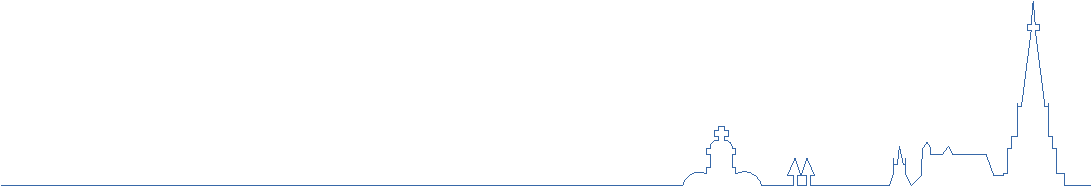
\includegraphics[width=9.0cm]{pics/sky_iuecol-rep.eps}}
\logo{\vspace{-0.3cm}\includegraphics[width=9.0cm]{pics/sky_iuecol.eps}}
%\pgfdeclareimage[height=1cm]{unilogo}{pics/TU_Signet_CMYK.eps}
%\usebackgroundtemplate{\includegraphics{pics/sky_iuecol.eps}}
% =========================================
\title{ViennaMesh\\A Highly Flexible Meshing Framework}

\author{\underline{Florian Rudolf}, Karl Rupp, and Siegfried Selberherr
}
\date{}
\institute[FEMTEC - Las Vegas, USA - May, 2013]{}

\titlegraphic{
   \begin{figure}[!ht]
   \vspace{-1.0cm}
   \begin{minipage}{1.5cm}
      \begin{center} 
         
\includegraphics[width=1.2cm]{pics/TU_Signet_CMYK.eps}
      \end{center}
   \end{minipage}
   \hfill
   \begin{minipage}{5.5cm}
      \begin{center}
      \scriptsize%\textsc{
      Institute for Microelectronics\\
      Technische Universit\"at Wien\\
      Vienna - Austria - Europe\\
      http:/$\negthinspace$/www.iue.tuwien.ac.at
      %}
      \end{center}
   \end{minipage}   
   \hfill   
   \begin{minipage}{1.5cm}
      \begin{center}
         \includegraphics[width=1.4cm]{pics/logo_px500.ps}
      \end{center}      
   \end{minipage}
\end{figure}
}


\begin{document}





\frame{\titlepage}

% ==============================================================================
\frame{
   \frametitle{Table of Contents}
   \tableofcontents
}

% ==============================================================================
\section{Introduction}
\subsection{}

% \begin{frame}[fragile]%[<+->]
%   \frametitle{Motivation}
%   
%   \begin{block}{Different applications require different meshing properties}
%     \begin{itemize} \footnotesize
%       \item Mesh quality is context-dependent
%     \end{itemize}
%   \end{block}
% 
%   \begin{block}{Different mesher generate meshes with different properties}
%     \begin{itemize} \itemsep0pt \footnotesize
%       \item Most meshing algorithms are only suitable for a specific set of applications
%     \end{itemize}
%   \end{block}
%   
%   \begin{block}{Simultaneous use of different meshing algorithms/libraries}
%     \begin{itemize} \itemsep0pt \footnotesize
%       \item Challenging due to incompatible data structures and interfaces\\
%       \item Many conversion functions are needed
%     \end{itemize}
%   \end{block}
% \end{frame}


\begin{frame}[fragile]%[<+->]
  \frametitle{Motivation}

  \begin{minipage}[t]{0.65\linewidth}
    \begin{block}{Different applications require different meshing properties}
      \begin{itemize} \footnotesize
        \item Mesh quality is context-dependent
      \end{itemize}
    \end{block}
  \end{minipage}
  \begin{minipage}[t]{0.30\linewidth}
    \begin{figure}
            \centering
            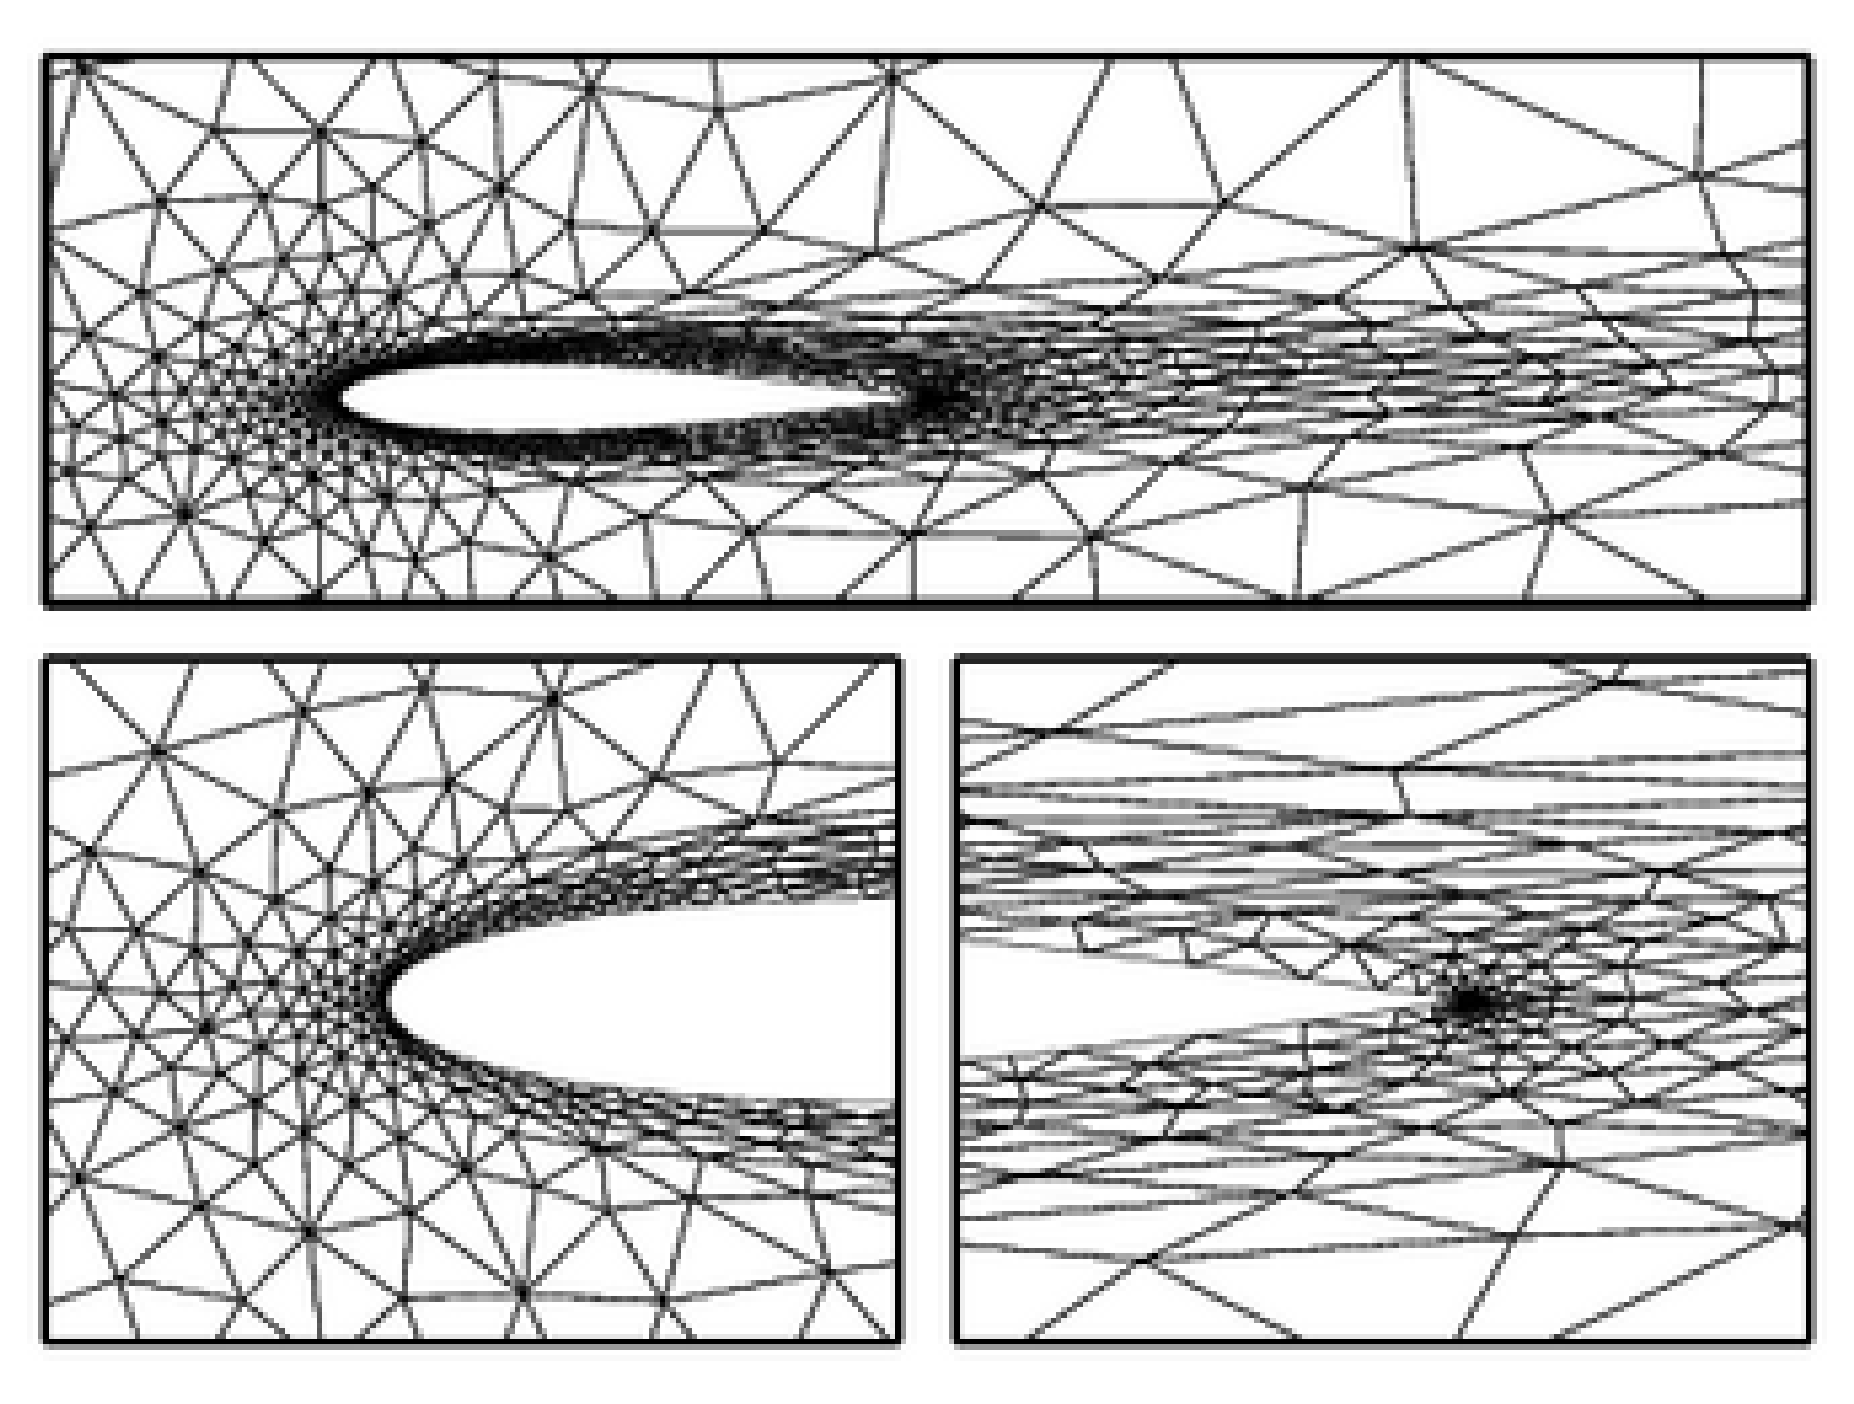
\includegraphics[scale=0.1]{figs/mesh_properties.eps}
    \end{figure}
  \end{minipage}
  
  \begin{block}{Different mesher generate meshes with different properties}
    \begin{itemize} \itemsep0pt \footnotesize
      \item Most meshing algorithms are only suitable for a specific set of applications
    \end{itemize}
  \end{block}
  
  \begin{block}{Simultaneous use of different meshing algorithms/libraries}
    \begin{itemize} \itemsep0pt \footnotesize
      \item Challenging due to incompatible data structures and interfaces
    \end{itemize}
  \end{block}
\end{frame}



\begin{frame}[fragile]%[<+->]
  \frametitle{Existing Frameworks and Libraries}

  \begin{block}{Often only one algorithm type is implemented}
    \begin{itemize} \itemsep0pt \footnotesize
      \item Usage is restricted to certain set of applications
    \end{itemize}
  \end{block}

  \begin{block}{Static data structure}
    \begin{itemize} \itemsep0pt \footnotesize
      \item Conversion from and to other formats is hard or even impossible
    \end{itemize}
  \end{block}
  
  \begin{block}{Static interface}
    \begin{itemize} \itemsep0pt \footnotesize
      \item Extensibility is hard or even impossible
    \end{itemize}
  \end{block}
\end{frame}



% ==============================================================================
\begin{frame}[fragile]%[<+->]
  \frametitle{Our Approach: ViennaMesh}

  \begin{block}{Open source C++ meshing framework}
    \begin{itemize} \itemsep0pt \footnotesize
      \item Multi-segment support
    \end{itemize}
  \end{block}

  \begin{block}{Based on a highly flexible data structure}
    \begin{itemize} \itemsep0pt \footnotesize
      \item Focus on abstract topology
    \end{itemize}
  \end{block}
  
  \begin{block}{Abstract concepts enable uniform interfaces}
    \begin{itemize} \itemsep0pt \footnotesize
      \item Generic programming
    \end{itemize}
  \end{block}
\end{frame}

% ==============================================================================
\section{The Framework}
\subsection{}

\begin{frame}[fragile]%[<+->]
  \frametitle{Library Details}

  \begin{block}{C++ library}
      \begin{itemize} \footnotesize
      \item Data structure and core functionality header-only
      \item C++11 support
      \end{itemize}   
  \end{block}
  
  \begin{block}{Interfaces to proven libraries}
      \begin{itemize} \footnotesize
      \item Meshing: Netgen, CGAL, VERDICT
      \item Statistics: Boost.Accumulators
      \item More to come: Tetgen, Triangle, Mesquite, ...
      \end{itemize}   
  \end{block}
\end{frame}



\begin{frame}[fragile]%[<+->]
  \frametitle{ViennaMesh - Topology}

  \begin{block}{Data structure is topology-driven}
    \begin{itemize} \footnotesize
      \item Abstract topology concept
      \item \textbf{Element, cell}, boundary element, co-boundary element
    \end{itemize}
  \end{block}
  
    \begin{figure}
            \centering
            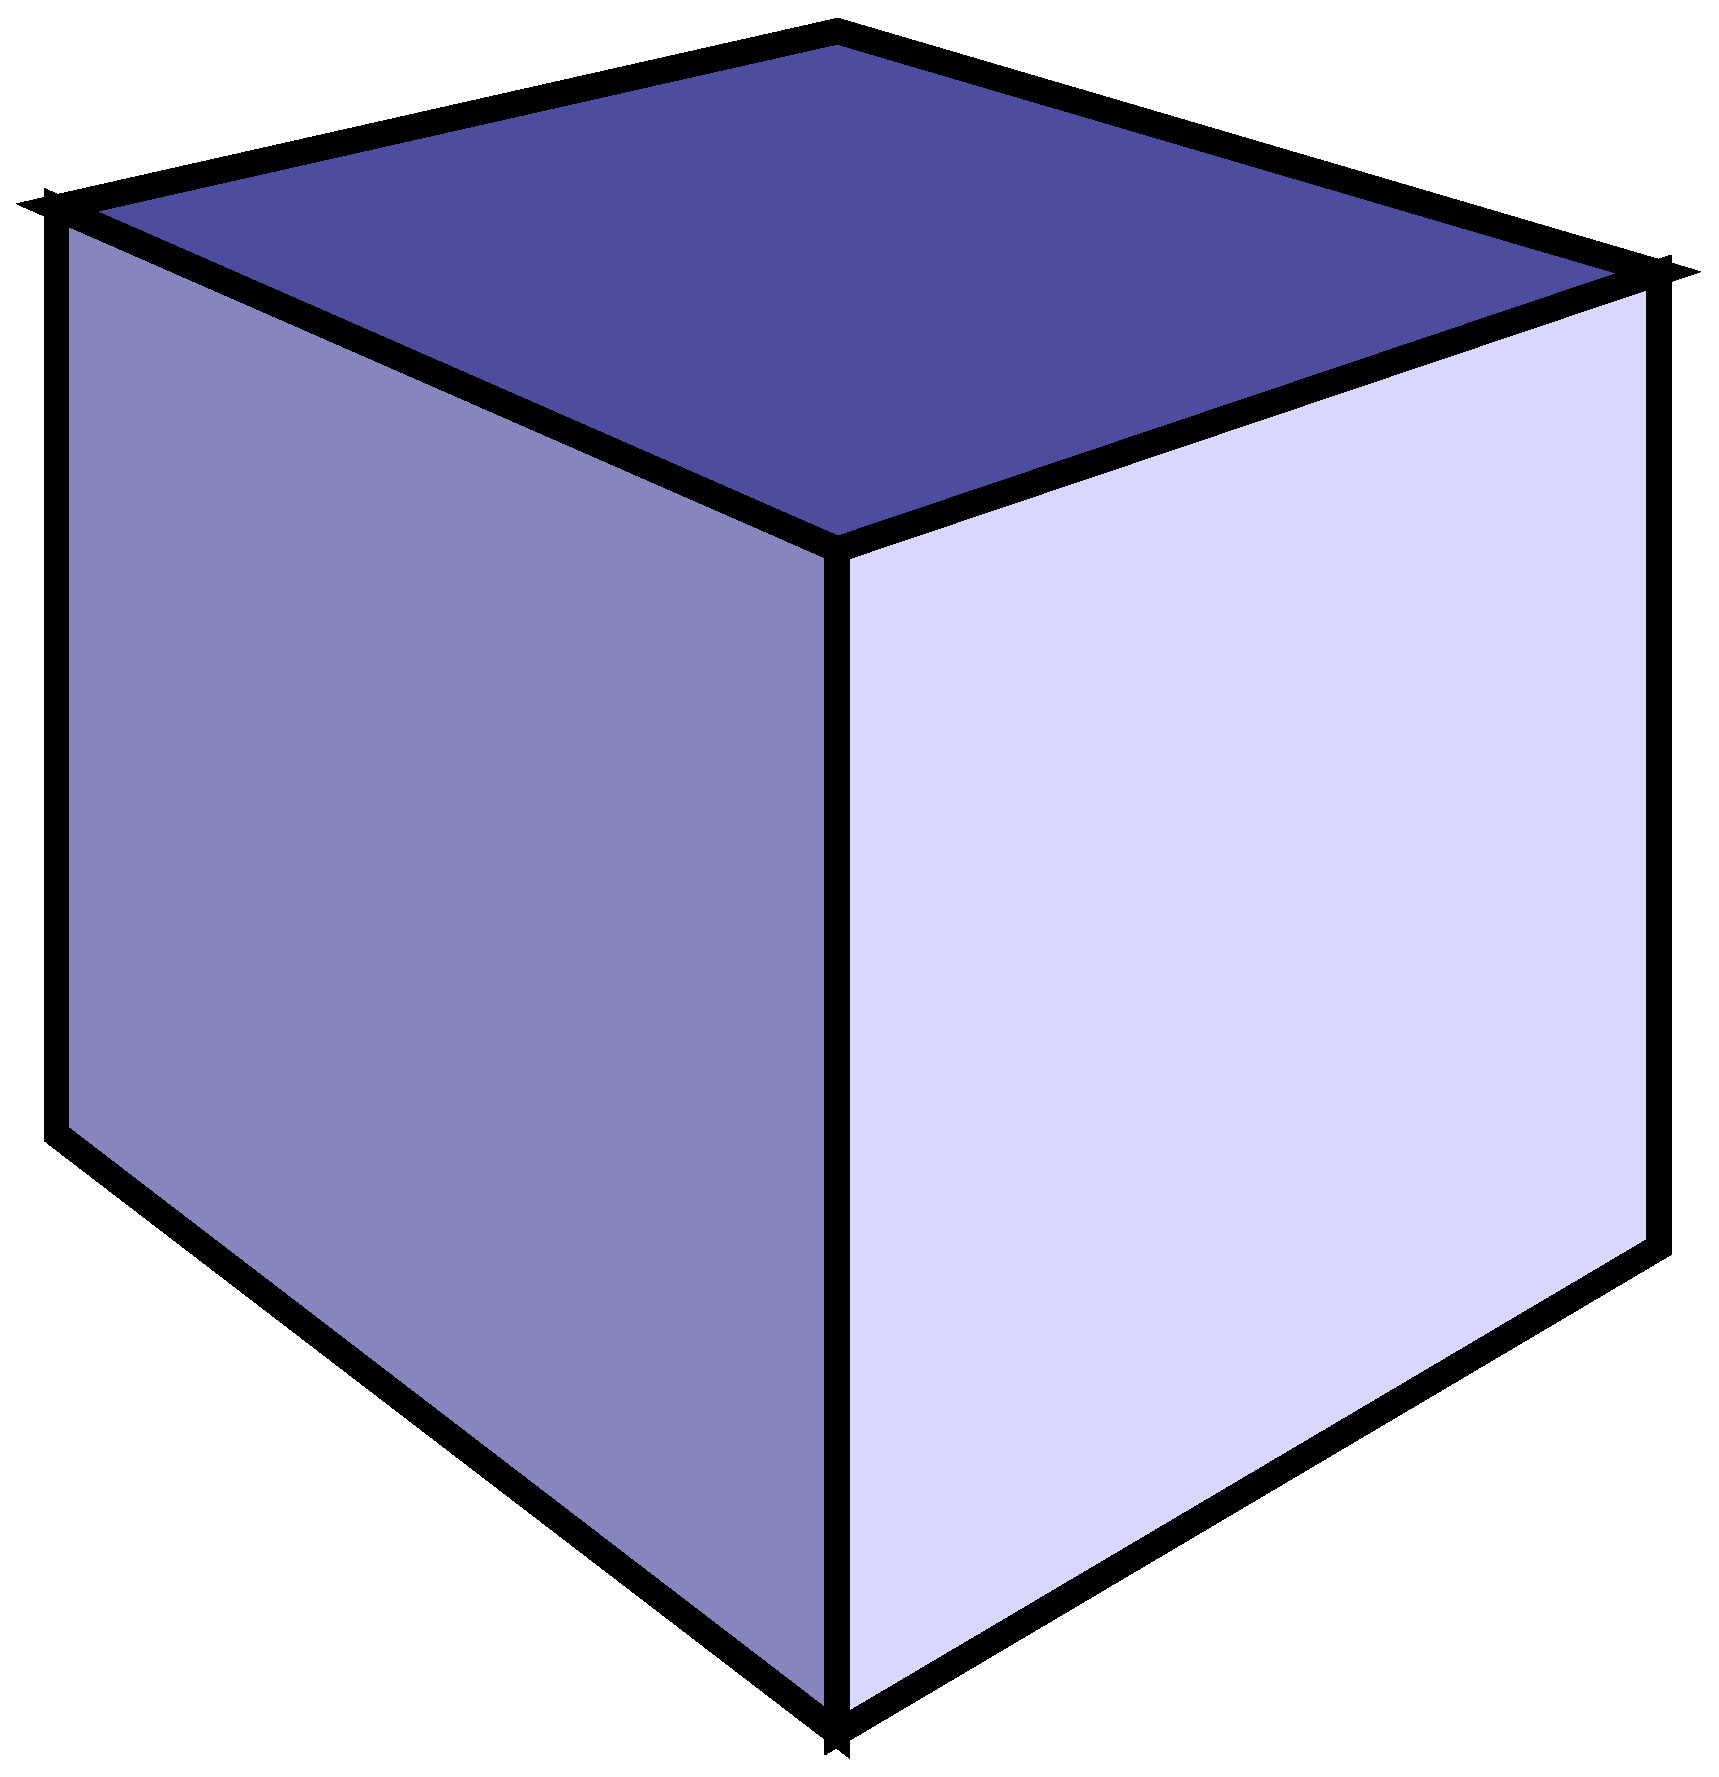
\includegraphics[scale=0.1]{figs/element.eps}
    \end{figure}
  
\end{frame}


\begin{frame}[fragile]%[<+->]
  \frametitle{ViennaMesh - Topology}

  \begin{block}{Data structure is topology-driven}
    \begin{itemize} \footnotesize
      \item Abstract topology concept
      \item Element, cell, \textbf{boundary element}, co-boundary element
    \end{itemize}
  \end{block}
  
    \begin{figure}
            \centering
            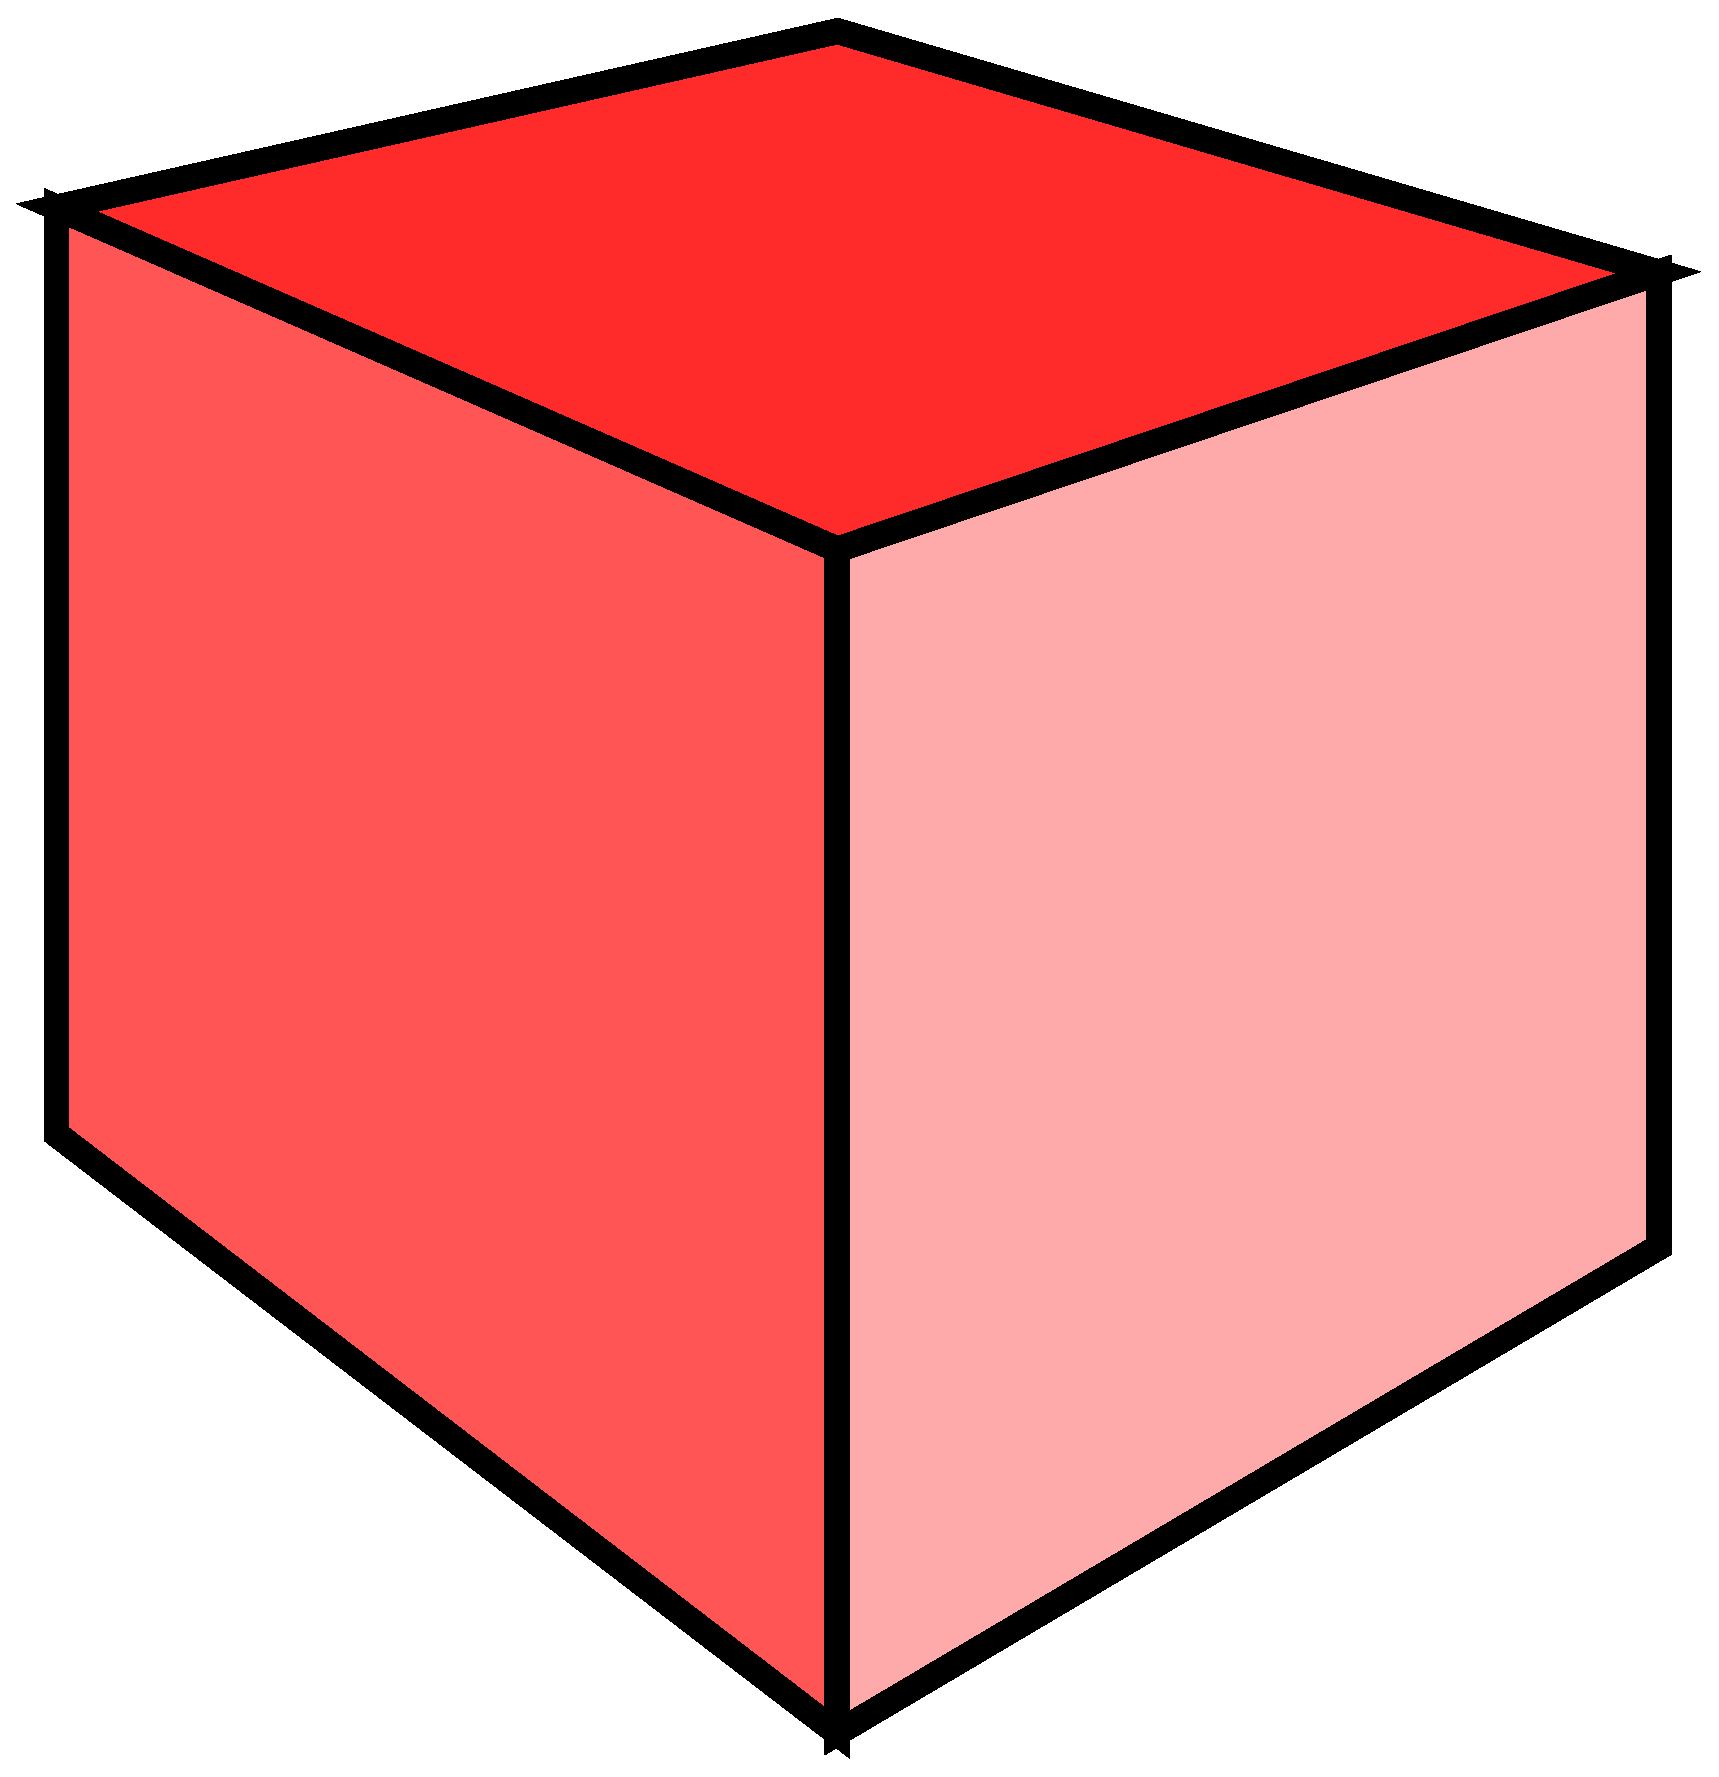
\includegraphics[scale=0.1]{figs/element_boundary_facet.eps}
    \end{figure}
  
\end{frame}


\begin{frame}[fragile]%[<+->]
  \frametitle{ViennaMesh - Topology}

  \begin{block}{Data structure is topology-driven}
    \begin{itemize} \footnotesize
      \item Abstract topology concept
      \item Element, cell, \textbf{boundary element}, co-boundary element
    \end{itemize}
  \end{block}
  
    \begin{figure}
            \centering
            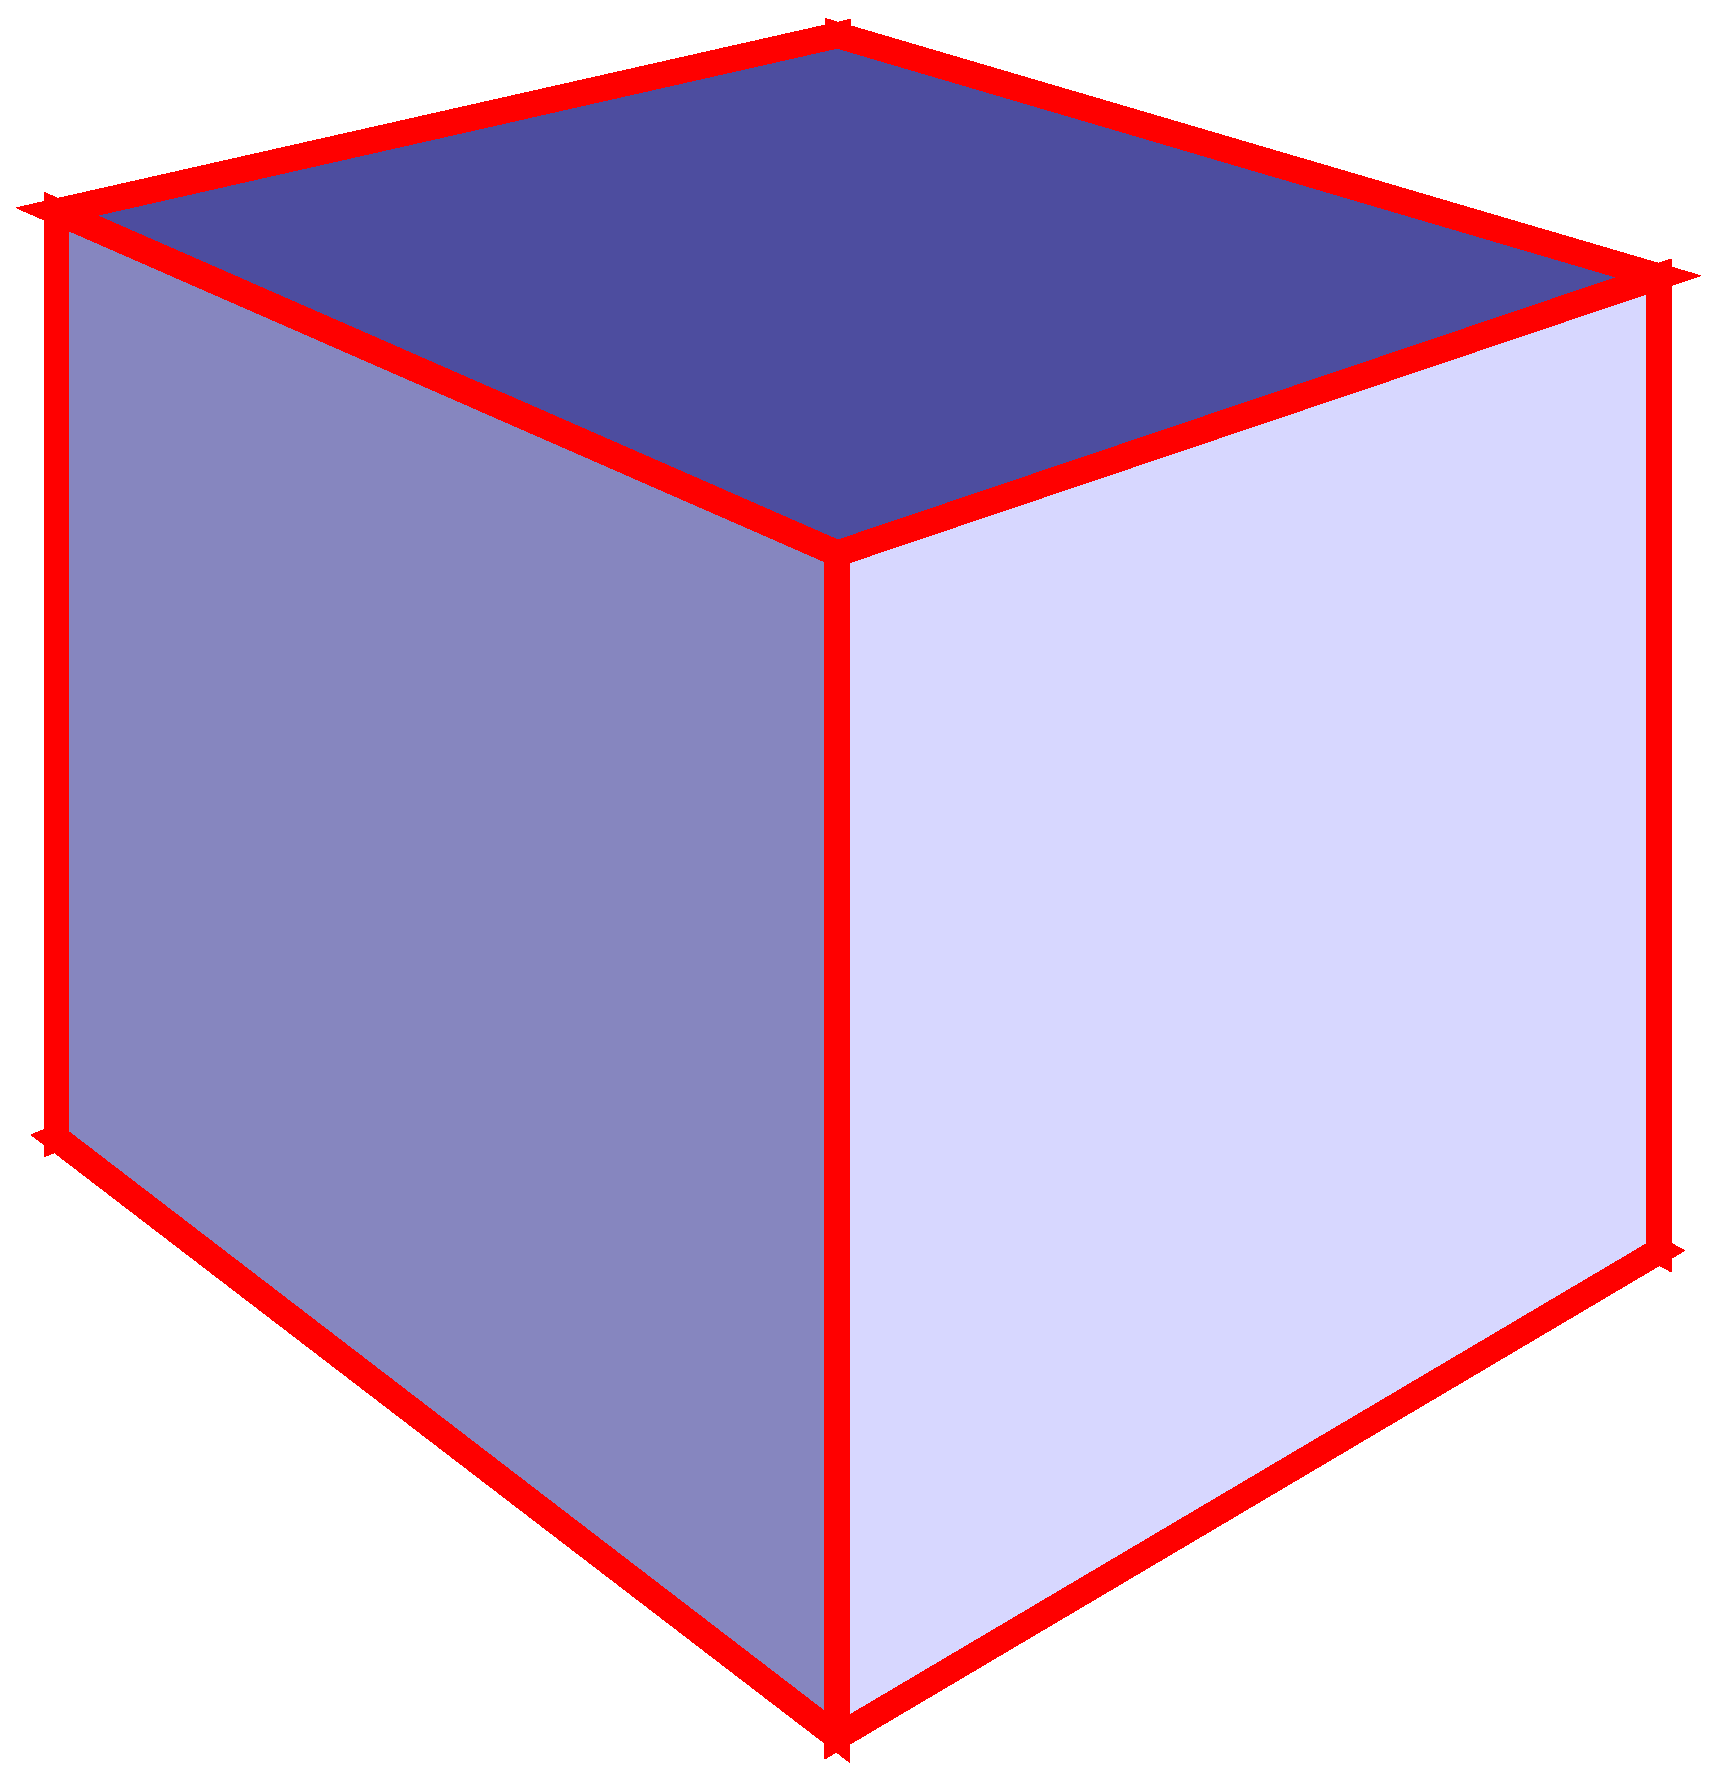
\includegraphics[scale=0.1]{figs/element_boundary_edge.eps}
    \end{figure}
  
\end{frame}


\begin{frame}[fragile]%[<+->]
  \frametitle{ViennaMesh - Topology}

  \begin{block}{Data structure is topology-driven}
    \begin{itemize} \footnotesize
      \item Abstract topology concept
      \item Element, cell, \textbf{boundary element}, co-boundary element
    \end{itemize}
  \end{block}
  
    \begin{figure}
            \centering
            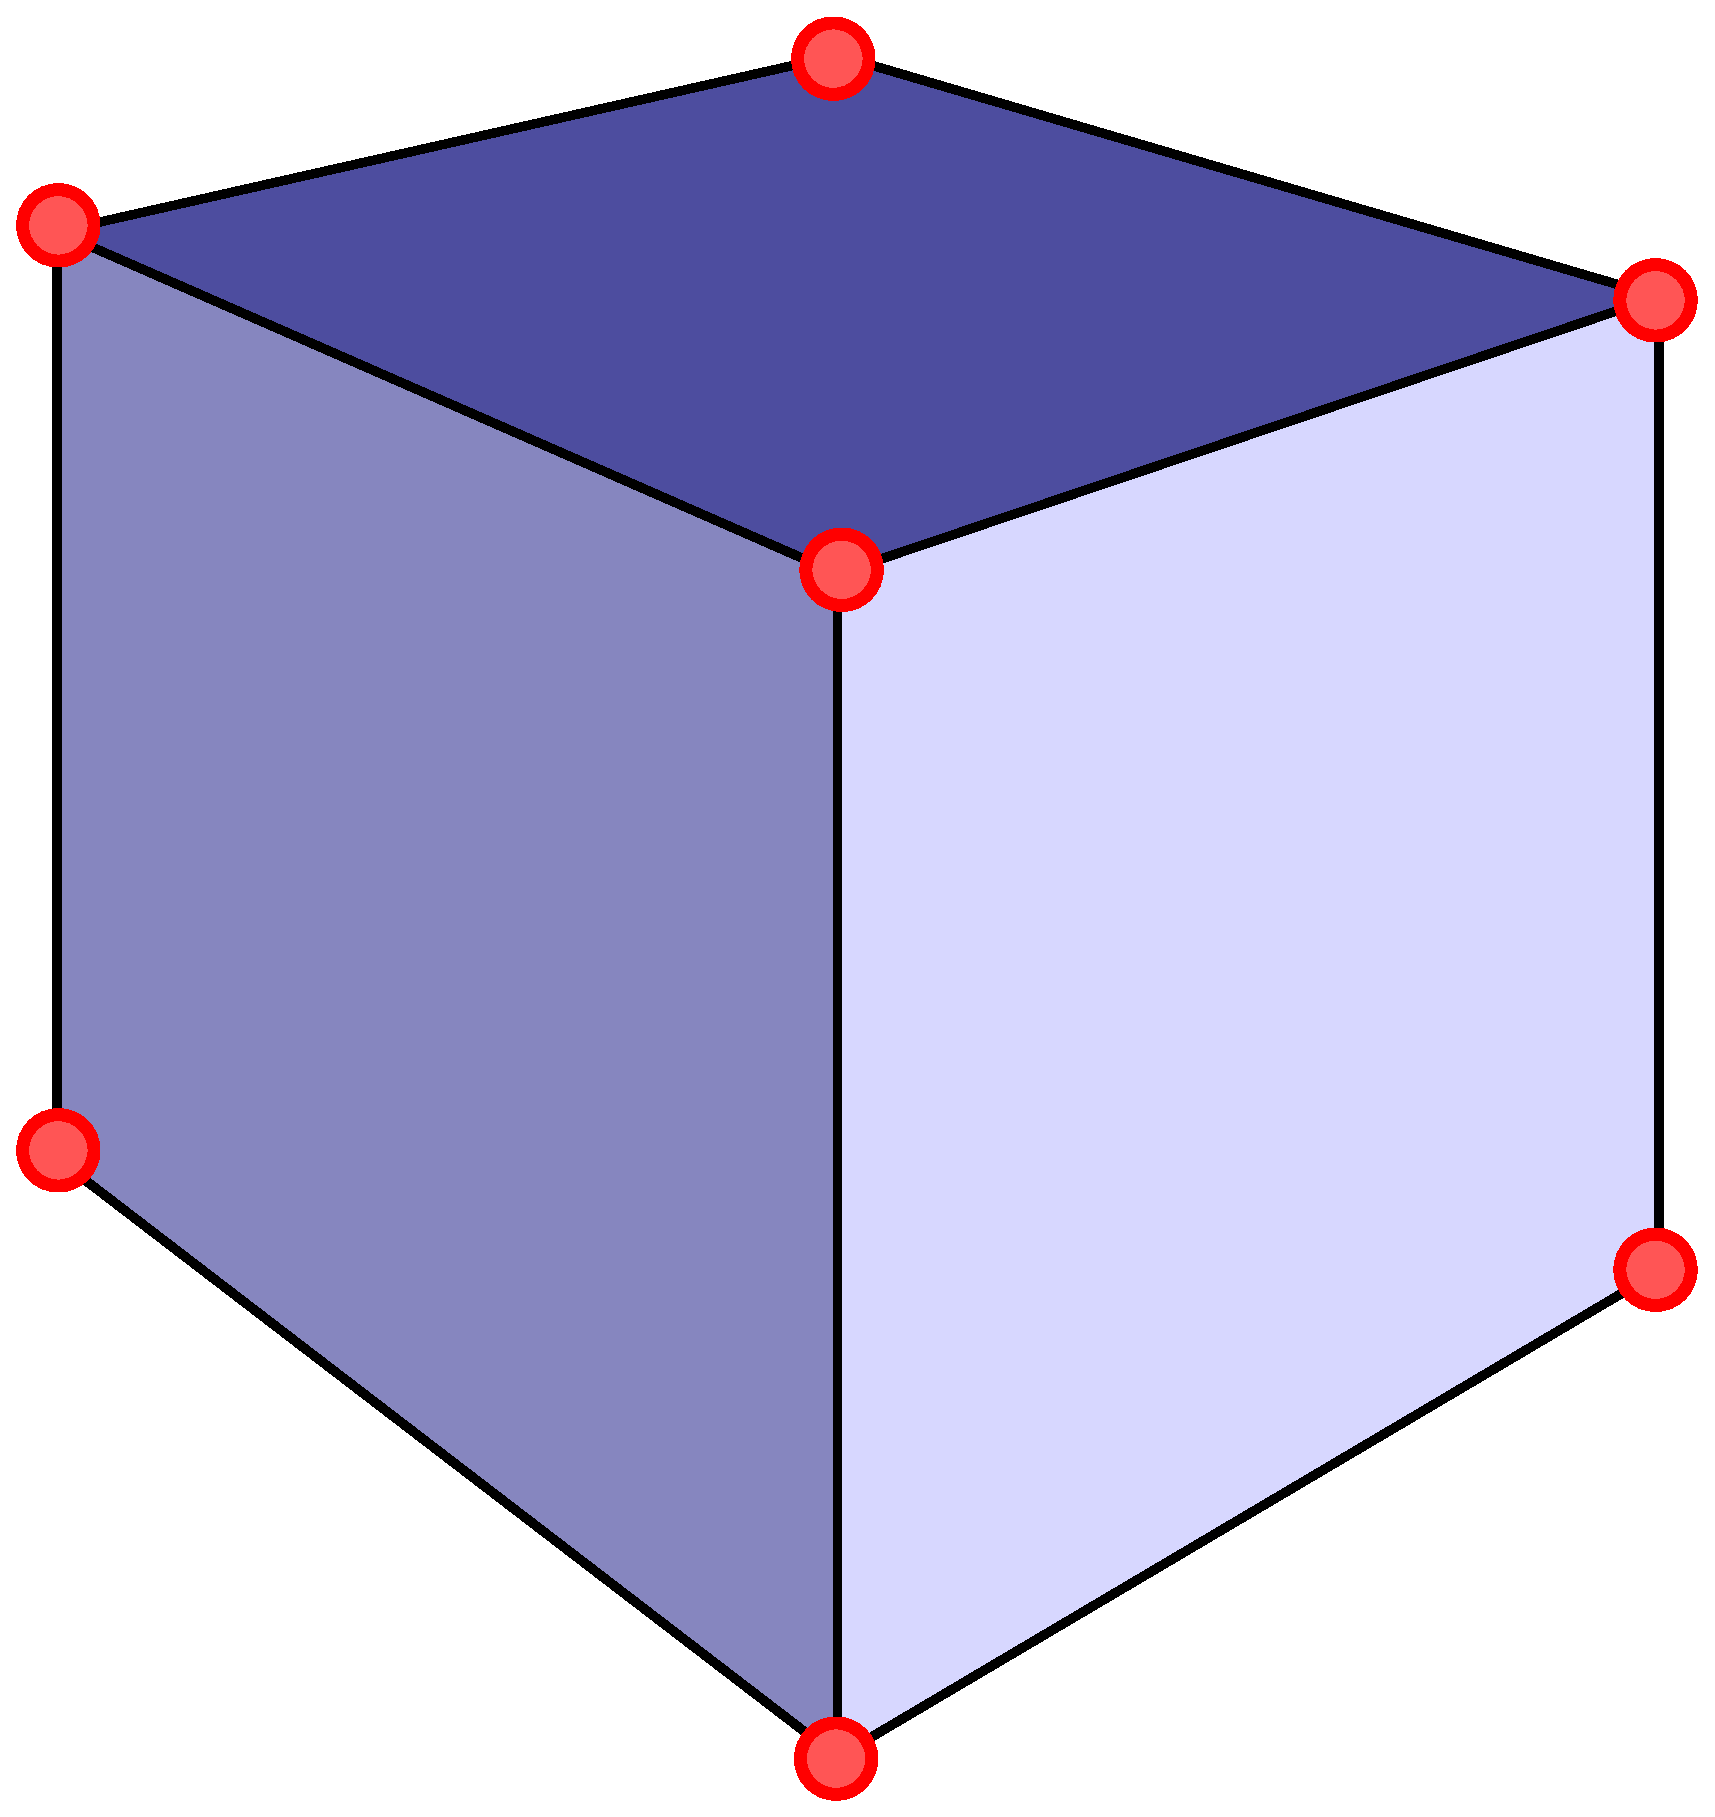
\includegraphics[scale=0.1]{figs/element_boundary_vertex.eps}
    \end{figure}
  
\end{frame}


\begin{frame}[fragile]%[<+->]
  \frametitle{ViennaMesh - Topology}

  \begin{block}{Data structure is topology-driven}
    \begin{itemize} \footnotesize
      \item Abstract topology concept
      \item Element, cell, boundary element, \textbf{co-boundary element}
      
    \end{itemize}
  \end{block}
  
    \begin{figure}
            \centering
            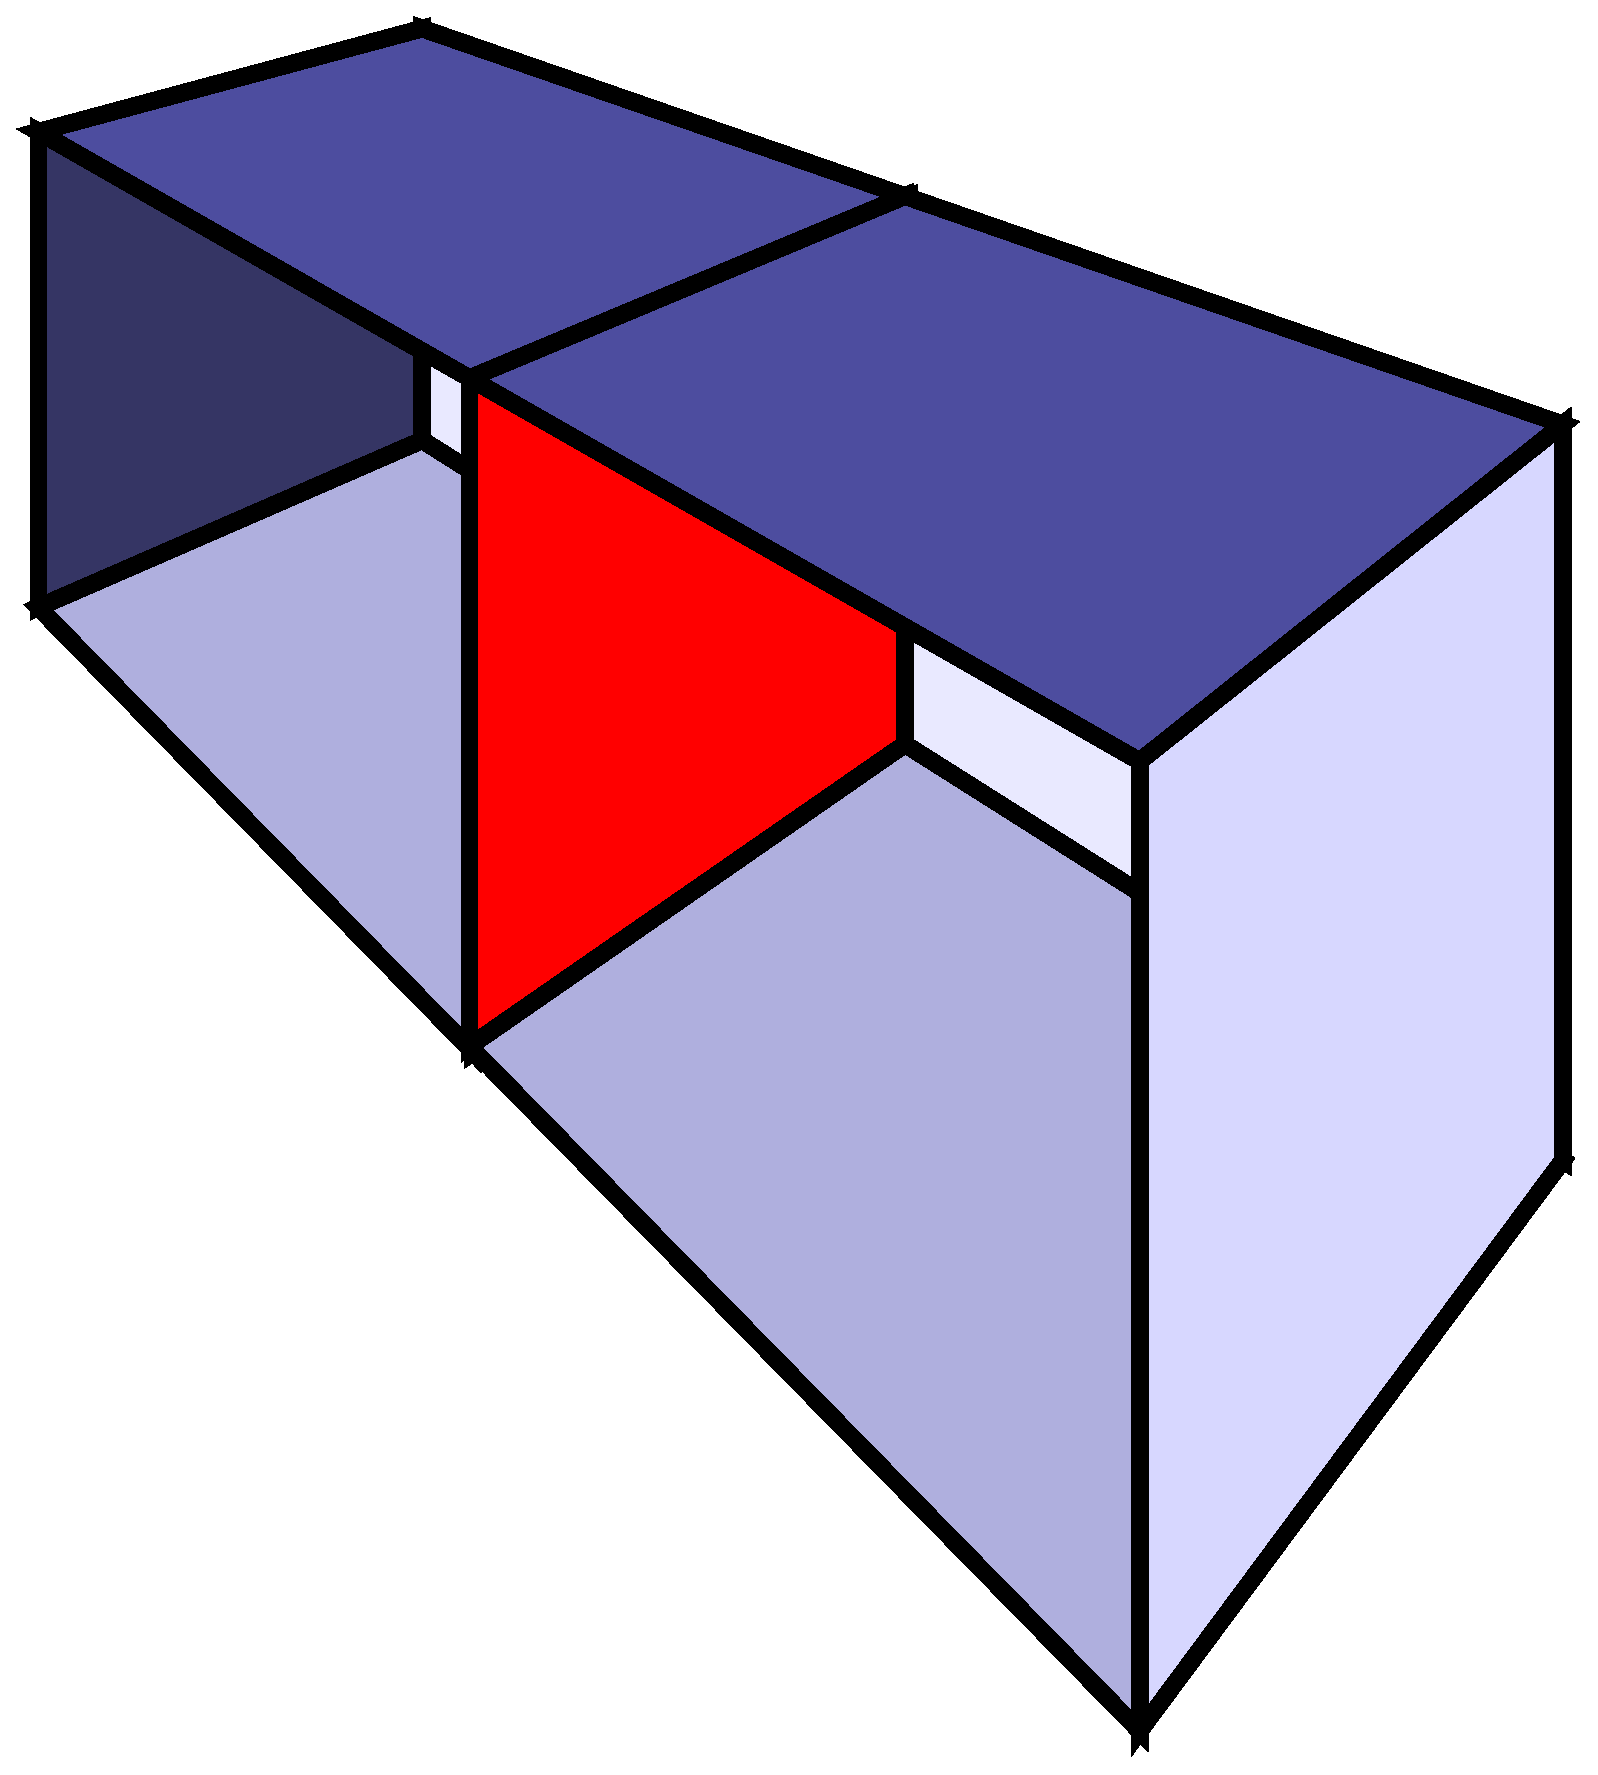
\includegraphics[scale=0.15]{figs/coboundary.eps}
    \end{figure}
  
\end{frame}




\begin{frame}[fragile]%[<+->]
  \frametitle{ViennaMesh - Data Structure}

  \begin{block}{Highly flexible topological structure}
    \begin{itemize} \footnotesize
      \item Simplices and hypercubes of arbitrary topological dimension
      \item Polygons and PLCs
    \end{itemize}
  \end{block}
  
  \begin{block}{Compile-time configuration using C++ templates}
    \begin{itemize} \footnotesize
      \item Better performance than run-time data structures
    \end{itemize}
  \end{block}

\end{frame}



\begin{frame}[fragile]%[<+->]
  \frametitle{ViennaMesh - Data Structure}

  \begin{block}{Topological complex}
    \begin{itemize} \footnotesize
      \item Set of elements
      \item Intersections of 2 elements $\rightarrow$ empty or another element
    \end{itemize}
  \end{block}
  
  \begin{block}{Topology and geometry are independent $\rightarrow$ separation}
    \begin{itemize} \footnotesize
      \item e.g. triangles in 3D space
    \end{itemize}
  \end{block}
  
  \begin{block}{Iterator interface is type-independent}
      \begin{itemize} \footnotesize
      \item Many algorithms can be written type-independently, e.g. data transfer
      \item Optimum: one source code for all element types
      \end{itemize}
  \end{block}

\end{frame}




\begin{frame}[fragile]%[<+->]
  \frametitle{ViennaMesh Data Structure Example - Data transfer}

  \begin{block}{Transfer data from triangle to vertex}
    \begin{itemize} \footnotesize
      \item value weighted with triangle volume
    \end{itemize}
  \end{block}
  
\begin{lstlisting}[linewidth=1.0 \textwidth]
for (auto v : viennagrid::vertices( domain ) )
{
  numeric_type weighted_value = 0, total_volume = 0;

  for ( auto t : viennagrid::triangles(domain, v) )
  {
    numeric_type current_volume = volume( domain, t );
    total_volume += current_volume;
    weighted_value += current_volume * value(t);
  }

  value(v) = weighted_value / total_volume;
}
\end{lstlisting}
\end{frame}



\begin{frame}[fragile]%[<+->]
  \frametitle{ViennaMesh Data Structure Example - Data transfer}

  \begin{block}{Type independent implementation}
    \begin{itemize} \footnotesize
      \item to\_tag and from\_tag specify the types
    \end{itemize}
  \end{block}
  
\begin{lstlisting}[linewidth=1.0 \textwidth]
|\color{blue}for (auto v : viennagrid::elements<to\_tag>( domain ) )|
{
  numeric_type weighted_value = 0, total_volume = 0;

  |\color{blue}for ( auto t : viennagrid::coboundary\_elements<from\_tag>(domain, v) )|
  {
    numeric_type current_volume = volume( domain, t );
    total_volume += current_volume;
    weighted_value += current_volume * value(t);
  }

  value(v) = weighted_value / total_volume;
}
\end{lstlisting}
\end{frame}



% \begin{frame}[fragile]%[<+->]
%   \frametitle{ViennaMesh Data Structure Example - Statistics}
% 
%   \begin{block}{Statistical analysis}
%       \begin{itemize} \footnotesize
%       \item Using Boost.Accumulators for statistic information
%       \end{itemize}
%   \end{block}
%   
% 
% \begin{lstlisting}[linewidth=1.0\textwidth]
% viennagrid::result_of::element_range<
%   DomainType, viennagrid::tetrahedron_tag>::type
%   ElementRange;
%        
% BoostAccumulatorType acc;       
%        
% ElementRange tetrahedrons = viennagrid::elements(domain);
% 
% for_each( tetrahedrons.begin(), tetrahedrons.end(),
%   [&domain, &acc](ElementRange::value_type & element)
%   { acc(viennamesh::aspect_ratio(domain, element)); } );
% \end{lstlisting}
% \end{frame}
% 
% 
% \begin{frame}[fragile]%[<+->]
%   \frametitle{ViennaMesh Data Structure Example - Statistics}
% 
%   \begin{block}{Statistical analysis}
%       \begin{itemize} \footnotesize
%       \item Using Boost.Accumulators for statistic information
%       \end{itemize}
%   \end{block}
%   
% 
% \begin{lstlisting}[linewidth=1.0\textwidth]
% viennagrid::result_of::element_range<
%   DomainType, viennagrid::tetrahedron_tag>::type
%   ElementRange;
%        
% |\color{blue}BoostAccumulatorType acc;|    
%        
% ElementRange tetrahedrons = viennagrid::elements(domain);
% 
% for_each( tetrahedrons.begin(), tetrahedrons.end(),
%   [&domain, &acc](ElementRange::value_type & element)
%   { acc(aspect_ratio(domain, element)); } );
% \end{lstlisting}
% \end{frame}
% 
% 
% \begin{frame}[fragile]%[<+->]
%   \frametitle{ViennaMesh Data Structure Example - Statistics}
% 
%   \begin{block}{Statistical analysis}
%       \begin{itemize} \footnotesize
%       \item C++11 lambda support
%       \end{itemize}
%   \end{block}
%   
% 
% \begin{lstlisting}[linewidth=1.0\textwidth]
% viennagrid::result_of::element_range<
%   DomainType, viennagrid::tetrahedron_tag>::type
%   ElementRange;
%        
% BoostAccumulatorType acc;       
%        
% ElementRange tetrahedrons = viennagrid::elements(domain);
% 
% for_each( domain.begin(), domain.end(),
%   |\color{blue}[\&domain, \&acc](ElementRange::value\_type \& element)|
%   |\color{blue}\{ acc(aspect\_ratio(domain, element)); \}| );
% \end{lstlisting}
% \end{frame}


\begin{frame}[fragile]%[<+->]
  \frametitle{ViennaMesh - Segment Support}
  
  \begin{minipage}[t]{0.48\linewidth}
    \begin{block}{Support for segments}
        \begin{itemize} \footnotesize
            \item Subsets of the mesh
            \item Preserve interfaces through\\meshing process
        \end{itemize}
    \end{block}
  \end{minipage}
  \begin{minipage}[t]{0.48\linewidth}
    \begin{figure}
            \centering
            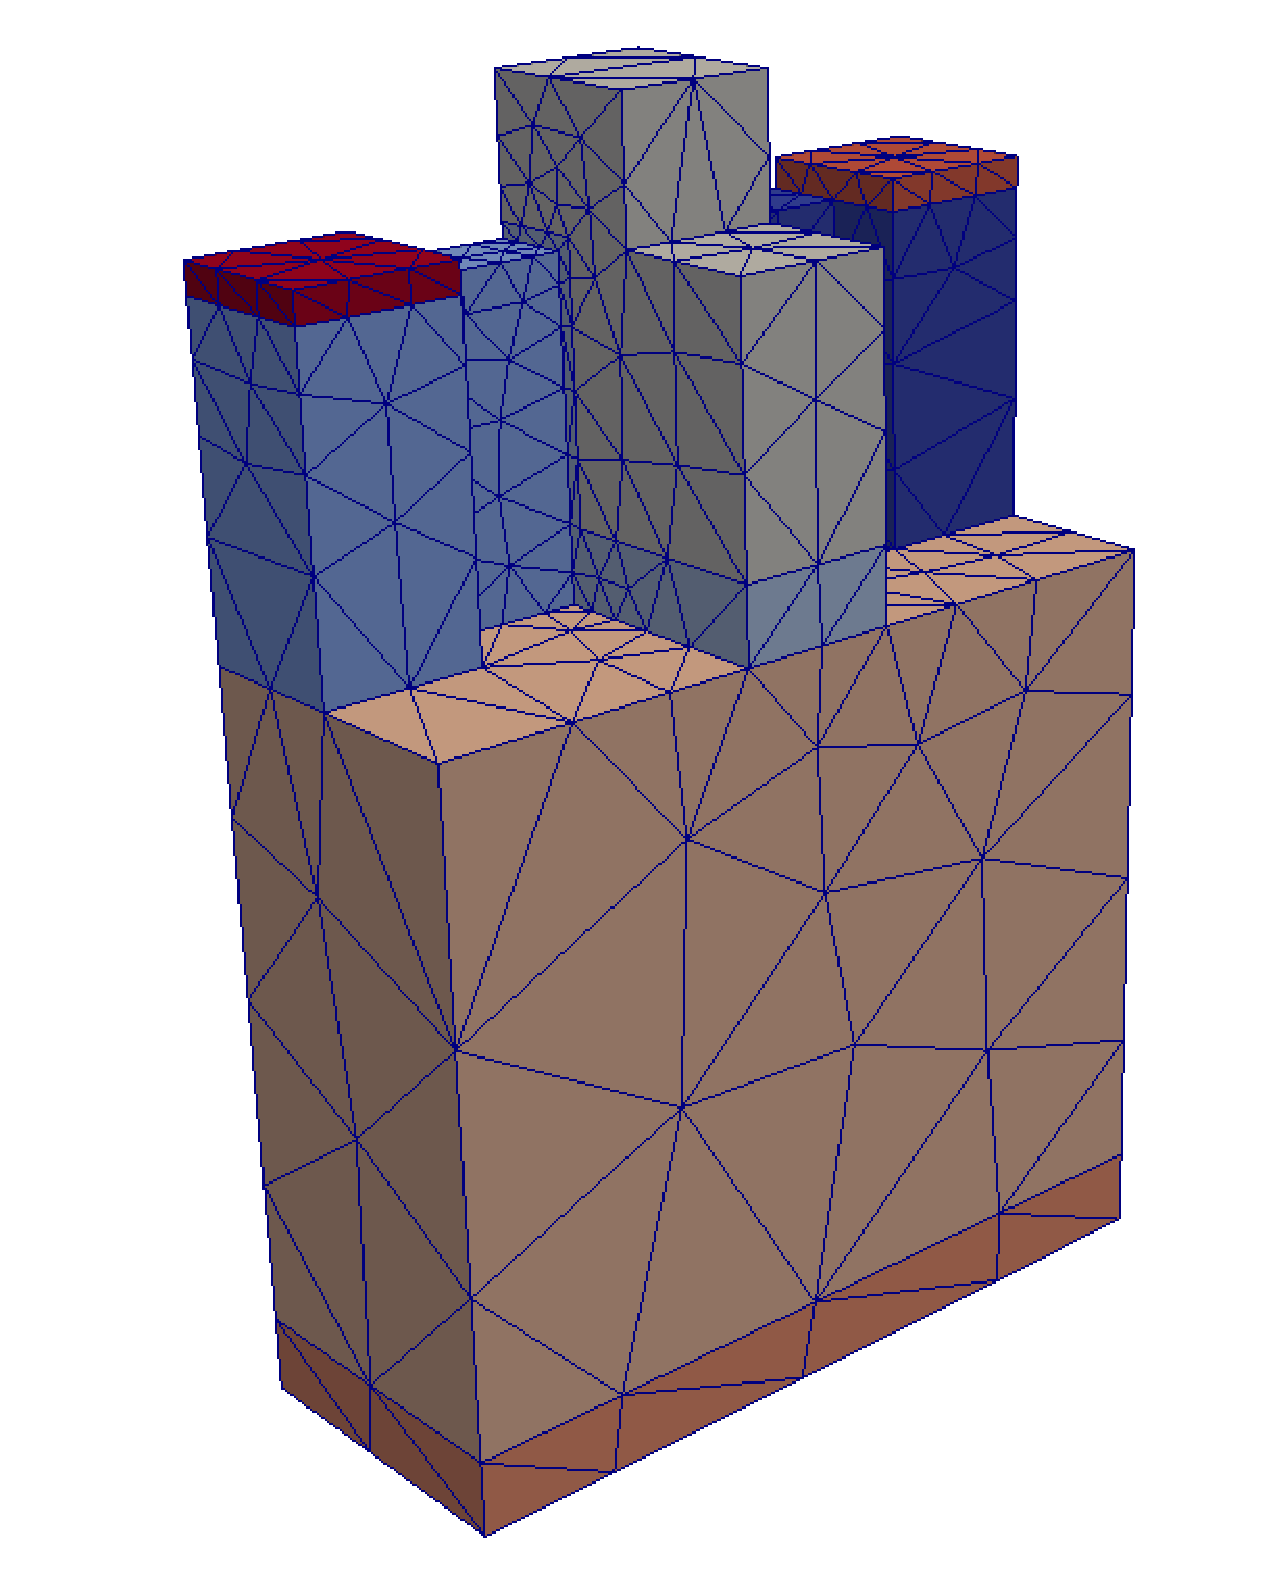
\includegraphics[scale=0.15]{figs/segments.eps}
    \end{figure}
  \end{minipage}

\end{frame}


\begin{frame}[fragile]%[<+->]
  \frametitle{ViennaMesh - Domain Concept}

  \begin{block}{External library support}
      \begin{itemize} \footnotesize
        \item External data structures
      \end{itemize}
  \end{block}  
  
  \begin{figure}
    \begin{subfigure}[b]{60mm}
      \centering
      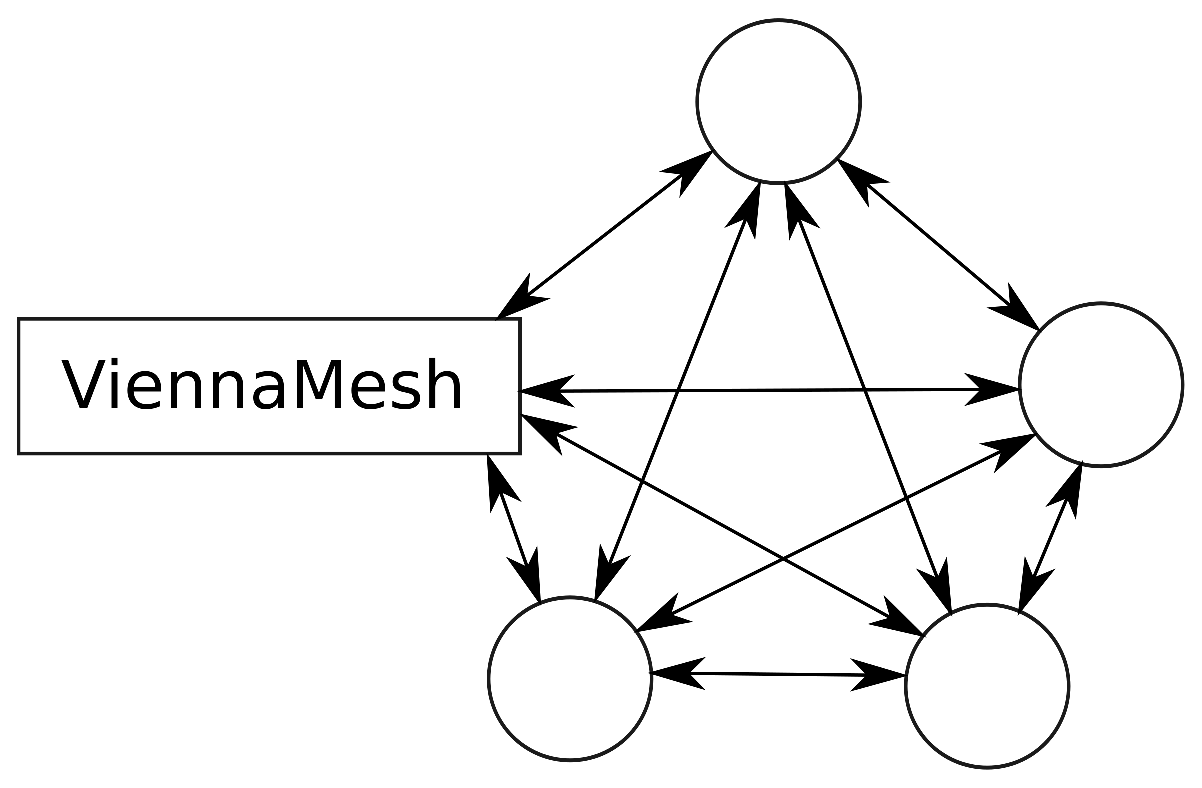
\includegraphics[scale=0.2]{figs/conversion.eps}
    \end{subfigure}
  \end{figure}

\end{frame}



\begin{frame}[fragile]%[<+->]
  \frametitle{ViennaMesh - Domain Concept}

  \begin{block}{External library support}
      \begin{itemize} \footnotesize
        \item External data structures
      \end{itemize}
  \end{block}  
  
  \begin{block}{Only 2 conversions per external data structure needed}
      \begin{itemize} \footnotesize
        \item From and to ViennaMesh
      \end{itemize}
  \end{block}
  
  \begin{figure}
    \begin{subfigure}[b]{60mm}
      \centering
      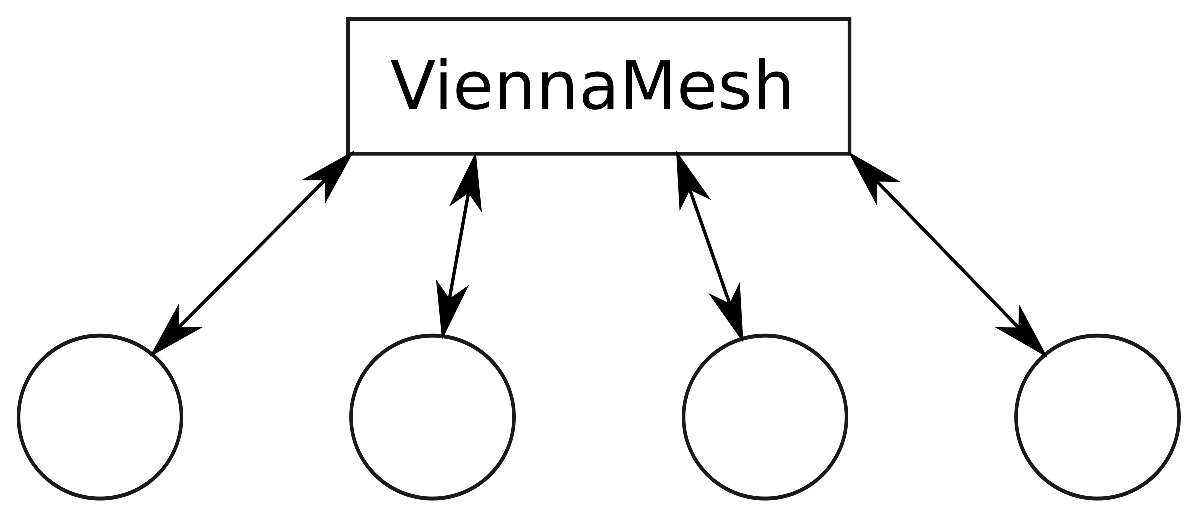
\includegraphics[scale=0.2]{figs/conversion_viennamesh.eps}
    \end{subfigure}
  \end{figure}

\end{frame}


  
  
\begin{frame}[fragile]%[<+->]
  \frametitle{ViennaMesh - Domain Concept}

  \begin{block}{Much less conversion functions needed}
    $\rightarrow$ $O(N)$ conversions instead of $O(N^2)$
  \end{block}
  
  \begin{block}{Conversion time about 1\% of the algorithm time}
    $\rightarrow$ no performance killer
  \end{block}

  \begin{block}{High configurability of topology}
    $\rightarrow$ ensures compatibility with other meshing data structures
  \end{block}
\end{frame}



\begin{frame}[fragile]%[<+->]
  \frametitle{ViennaMesh - Supported Algorithms}

  \begin{block}{Externally provided algorithms}
      \begin{itemize} \footnotesize
      \item Netgen: Triangular hull $\rightarrow$ Tetrahedron, multi-segment support
      \item CGAL: PLC $\rightarrow$ Triangular hull
      \item CGAL: Triangular hull $\rightarrow$ Tetrahedron
      \end{itemize}
  \end{block}

  \begin{block}{Internally provided algorithms}
    
      \begin{itemize} \footnotesize
      \item Multi-segment hull refinement
      \item Seed point segmenting
      \item Hull/Geometry extraction
      \end{itemize}
  \end{block}

\end{frame}



\begin{frame}[fragile]%[<+->]
  \frametitle{ViennaMesh - Meshing Algorithms}

  \begin{block}{External and internal algorithms share common interface}
      \begin{itemize} \footnotesize
        \item data structure conversion if needed
      \end{itemize}
  \end{block}

\begin{lstlisting}[linewidth=1.0\textwidth]
InputDomainType  input_domain;
OutputDomainType output_domain;
viennamesh::result_of::settings<algorithm_tag>::type
                settings;
                
settings.cell_size = 1.0;

viennamesh::run_algo< algorithm_tag >(
    |\color{blue}input\_domain|,
    |\color{blue}output\_domain|,
    settings);
\end{lstlisting}

\end{frame}



\begin{frame}[fragile]%[<+->]
  \frametitle{ViennaMesh - Meshing Algorithms}

  \begin{block}{External and internal algorithms share common interface}
      \begin{itemize} \footnotesize
        \item Easy exchangeability of algorithms
      \end{itemize}
  \end{block}

\begin{lstlisting}[linewidth=1.0\textwidth]
InputDomainType  input_domain;
OutputDomainType output_domain;
viennamesh::result_of::settings< |\color{blue}algorithm\_tag| >::type
                settings;

settings.cell_size = 1.0;
                
viennamesh::run_algo< |\color{blue}algorithm\_tag| >(
    input_domain,
    output_domain,
    settings);
\end{lstlisting}

\end{frame}





\section{Use Case}
\subsection{}

\begin{frame}[fragile]%[<+->]
  \frametitle{Use Case - Adaptive Finite Element/Volume Method}
  
    \begin{figure}
            \centering
            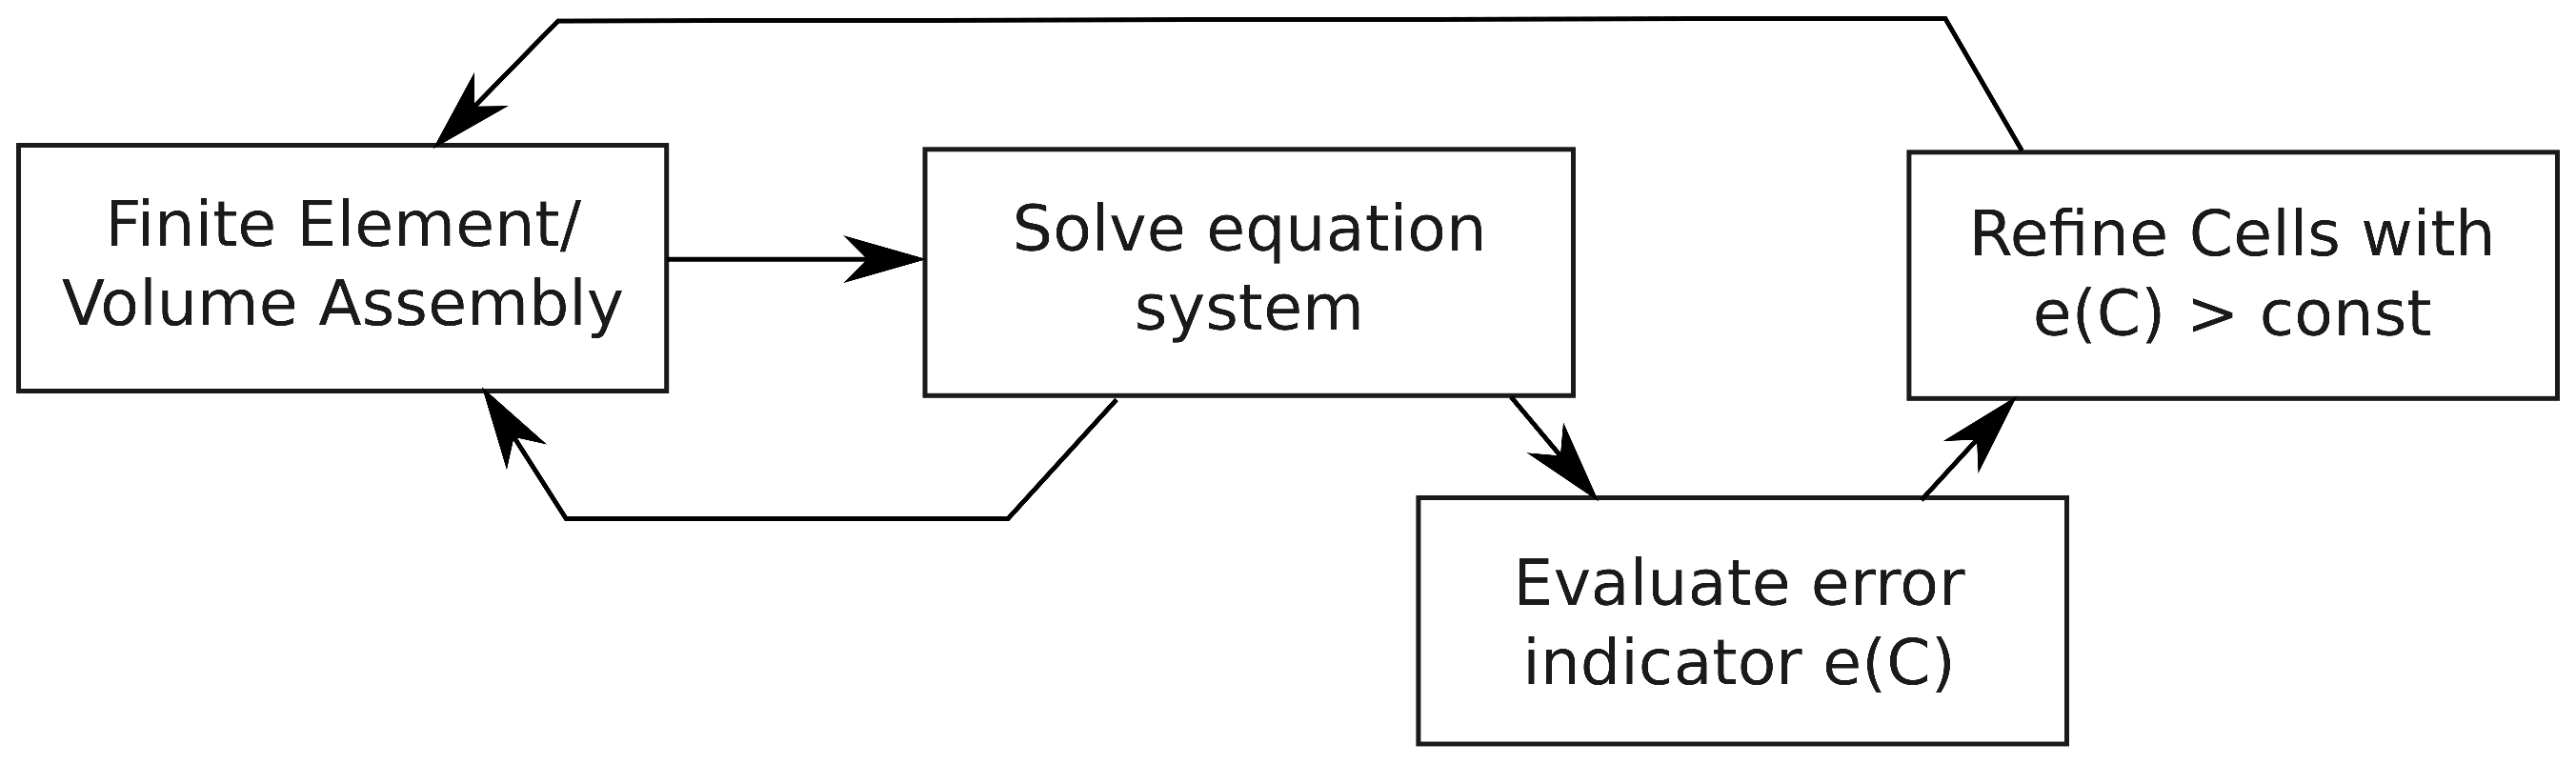
\includegraphics[scale=0.2]{figs/use_case_flowchart.eps}
    \end{figure}
  
  \begin{block}{Adaptive Loop}
      \begin{itemize} \footnotesize
      \item Error indicator $e(C) := max_{A \in \textnormal{neighbour}(C) } \{ | \textnormal{value}(A) - \textnormal{value}(C) |  \}  $
      \item Cells with $ e(C) > \textnormal{const} $ are refined
      \end{itemize}
  \end{block}

\end{frame}


\begin{frame}[fragile]%[<+->]
  \frametitle{Use Case - Drift Diffusion on 3D MOSFET Transistor}
  
  \begin{block}{Drift Diffusion}
    \vspace{-0.7cm}
    \begin{eqnarray*}
      \nabla \cdot ( \epsilon \nabla \psi ) & = & q ( (n-N_D) - (p-N_A) )\\
      \nabla \cdot ( D \nabla n - \mu n \nabla \psi ) & = & 0\\
      \nabla \cdot ( D \nabla p + \mu p \nabla \psi ) & = & 0
    \end{eqnarray*}
  \end{block}
  
  \begin{block}{Drift Diffusion on 3D MOSFET transistor}
      \begin{itemize} \footnotesize
      \item Using Finite Element/Volume assembly
      \item Starting mesh: 3200 cells
      \end{itemize}
  \end{block}

  \footnotesize
  J J H Miller et al, Report on Progress in Physics, 1999
  
\end{frame}



\begin{frame}[fragile]%[<+->]
  \frametitle{Drift Diffusion on 3D MOSFET Transistor}
  
\begin{figure}
        \centering
        \begin{subfigure}[b]{60mm}
                \centering
                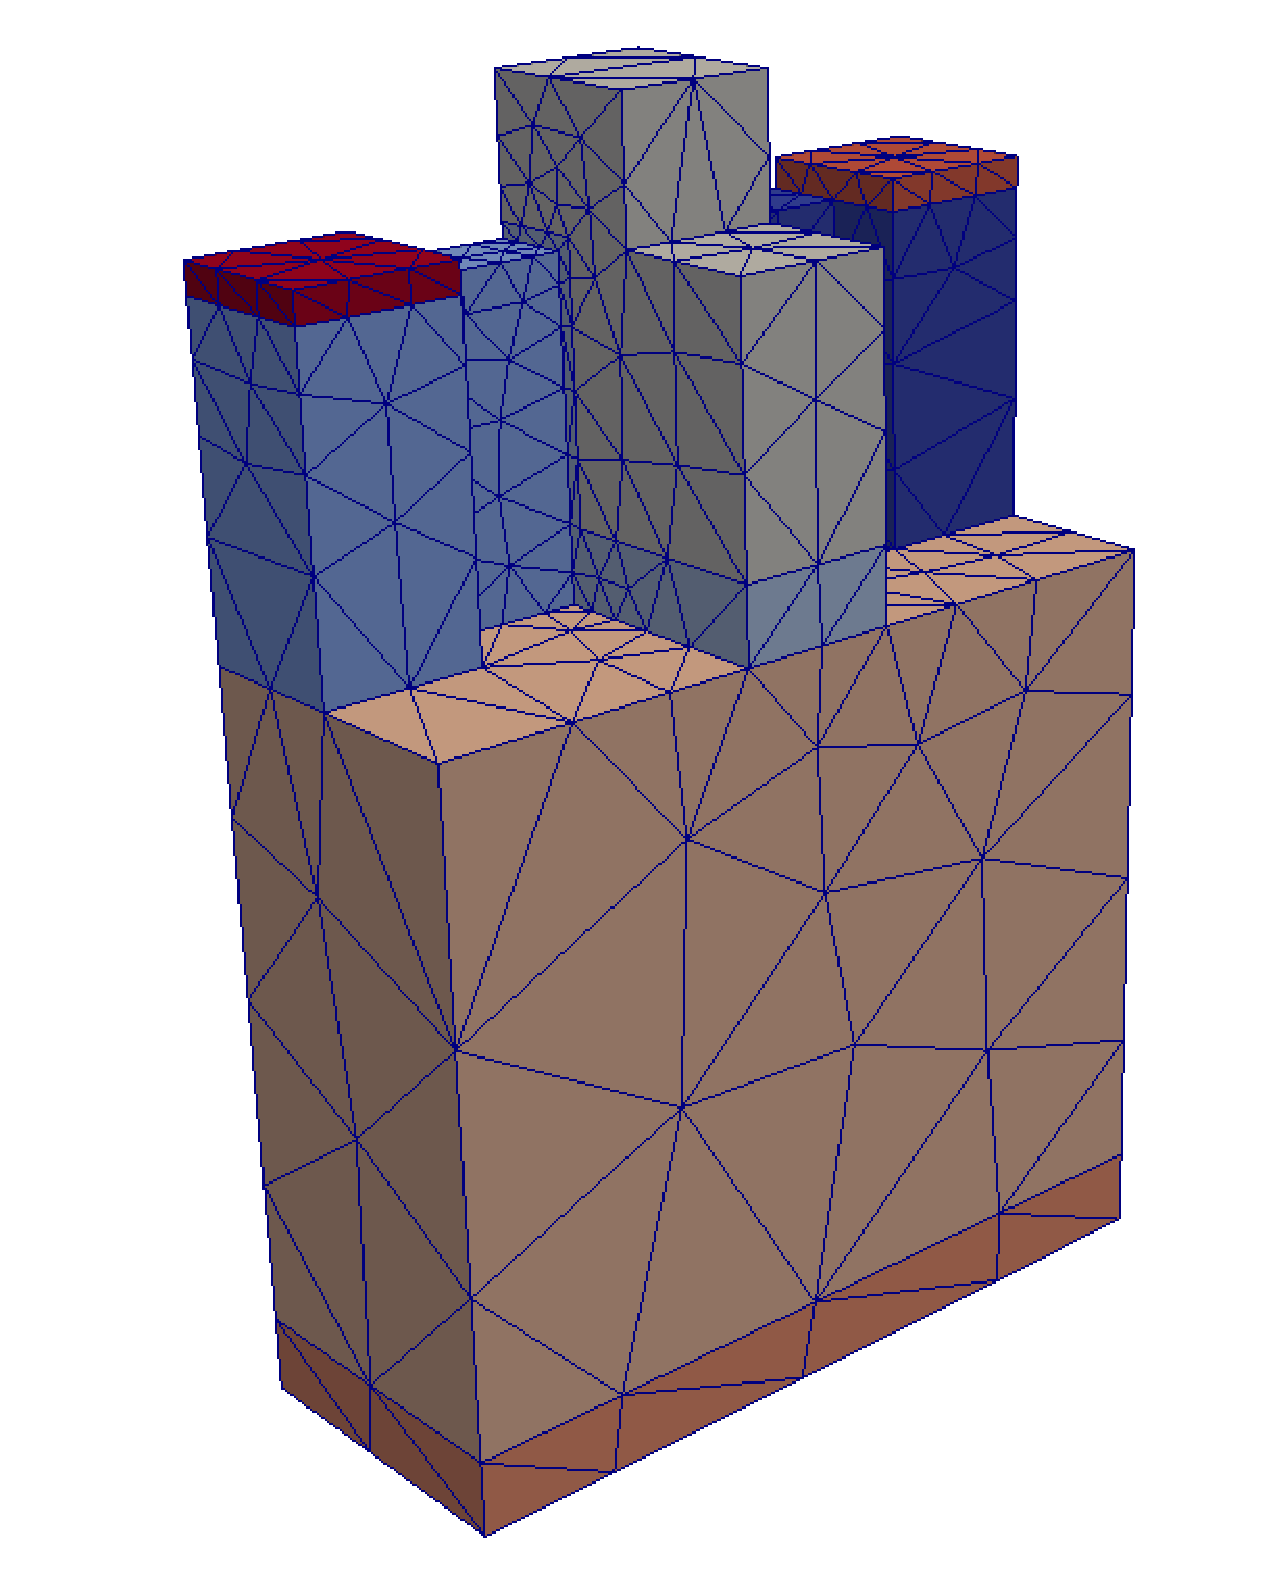
\includegraphics[scale=0.2]{figs/segments.eps}
                \caption*{Initial mesh with 3200 cells}
        \end{subfigure}%
\end{figure}
   
\end{frame}



\begin{frame}[fragile]%[<+->]
  \frametitle{Refinement - First Iteration}
  
\begin{figure}
        \centering
        \begin{subfigure}[b]{45mm}
                \centering
                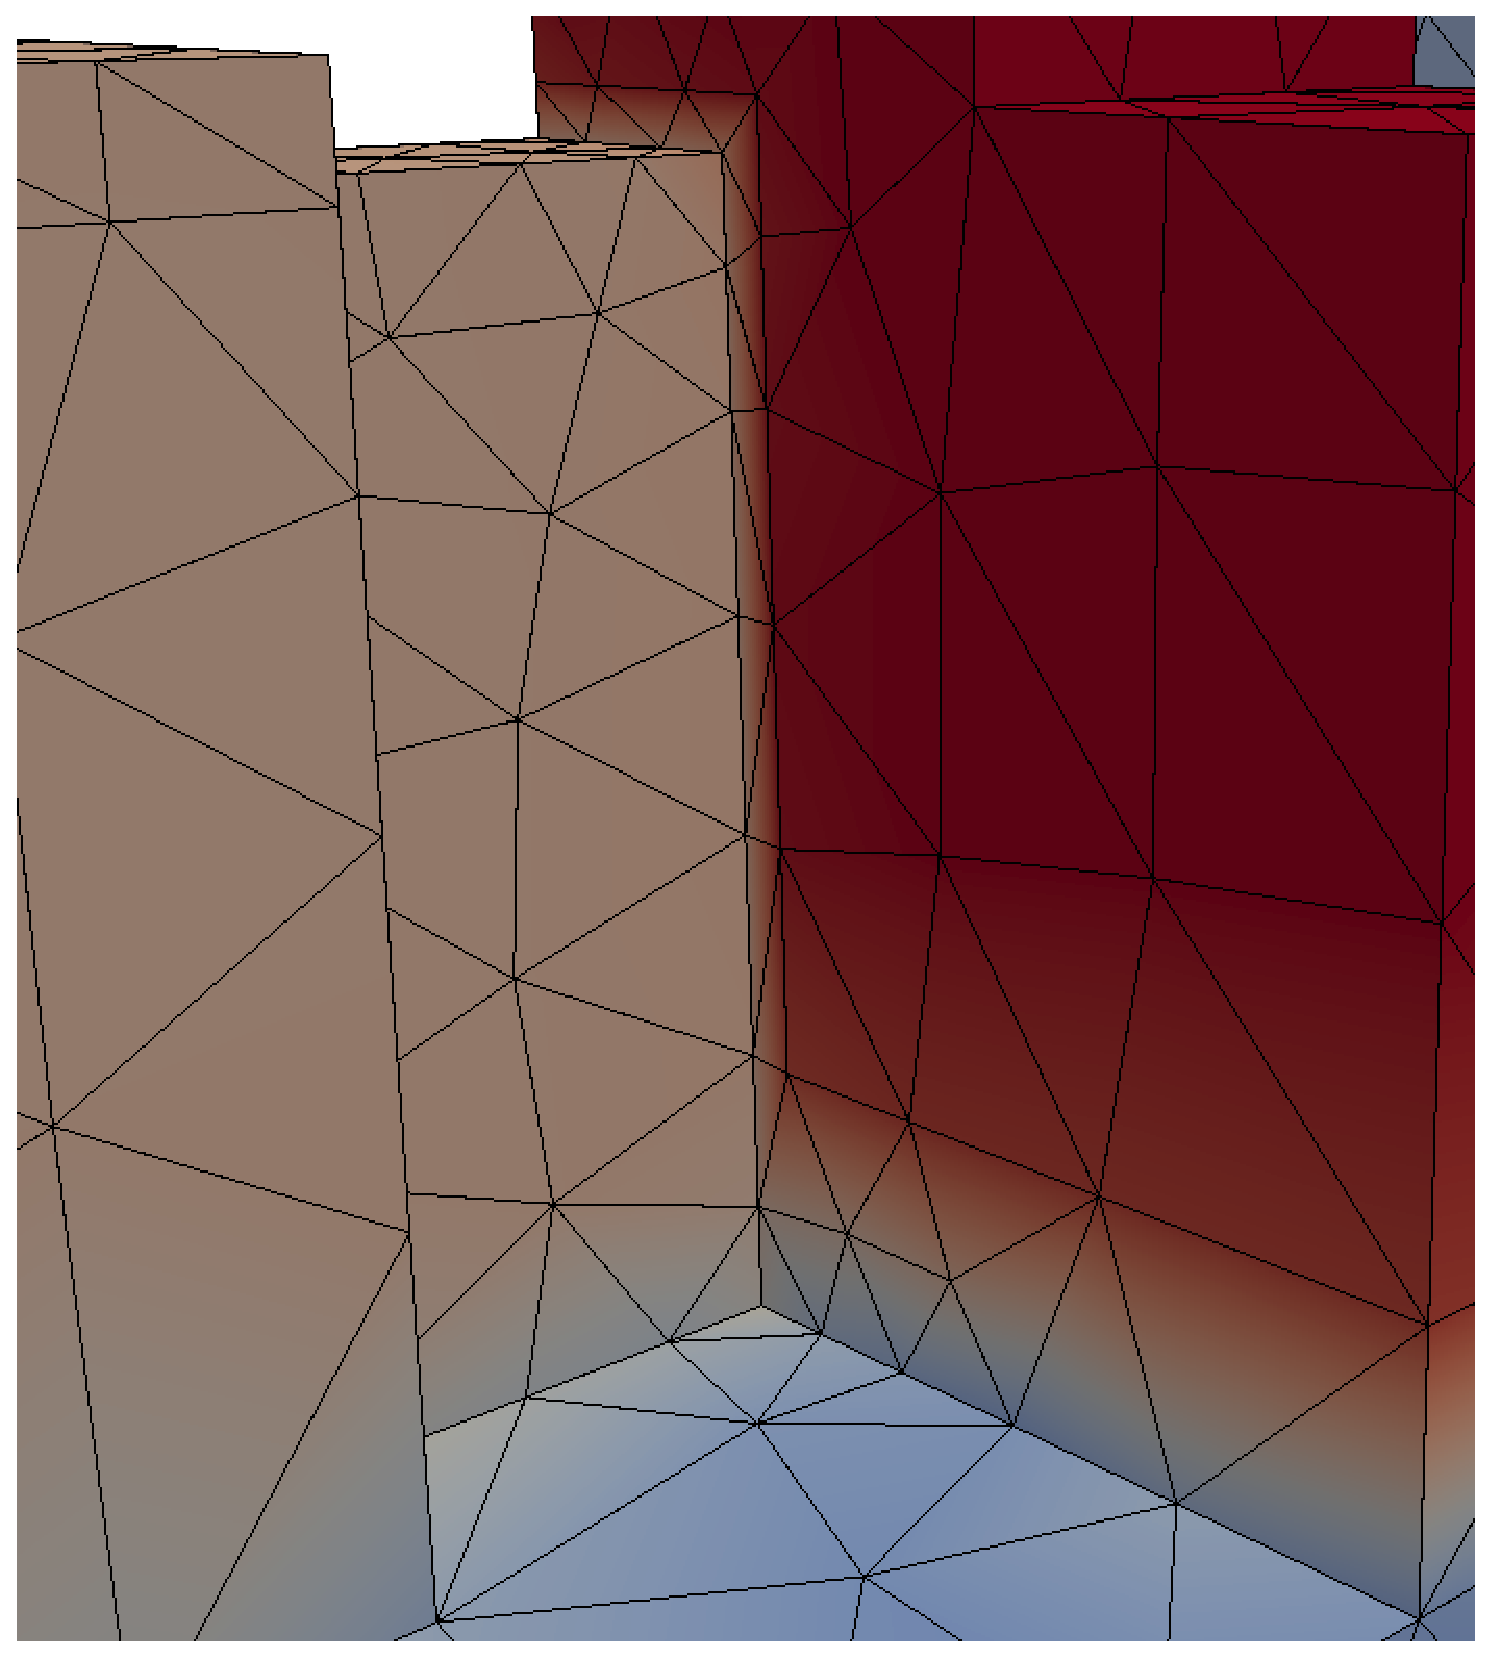
\includegraphics[scale=0.2]{figs/iter0_local.eps}
                \caption*{Potential}
        \end{subfigure}%
        \hspace{10mm}
        \begin{subfigure}[b]{45mm}
                \centering
                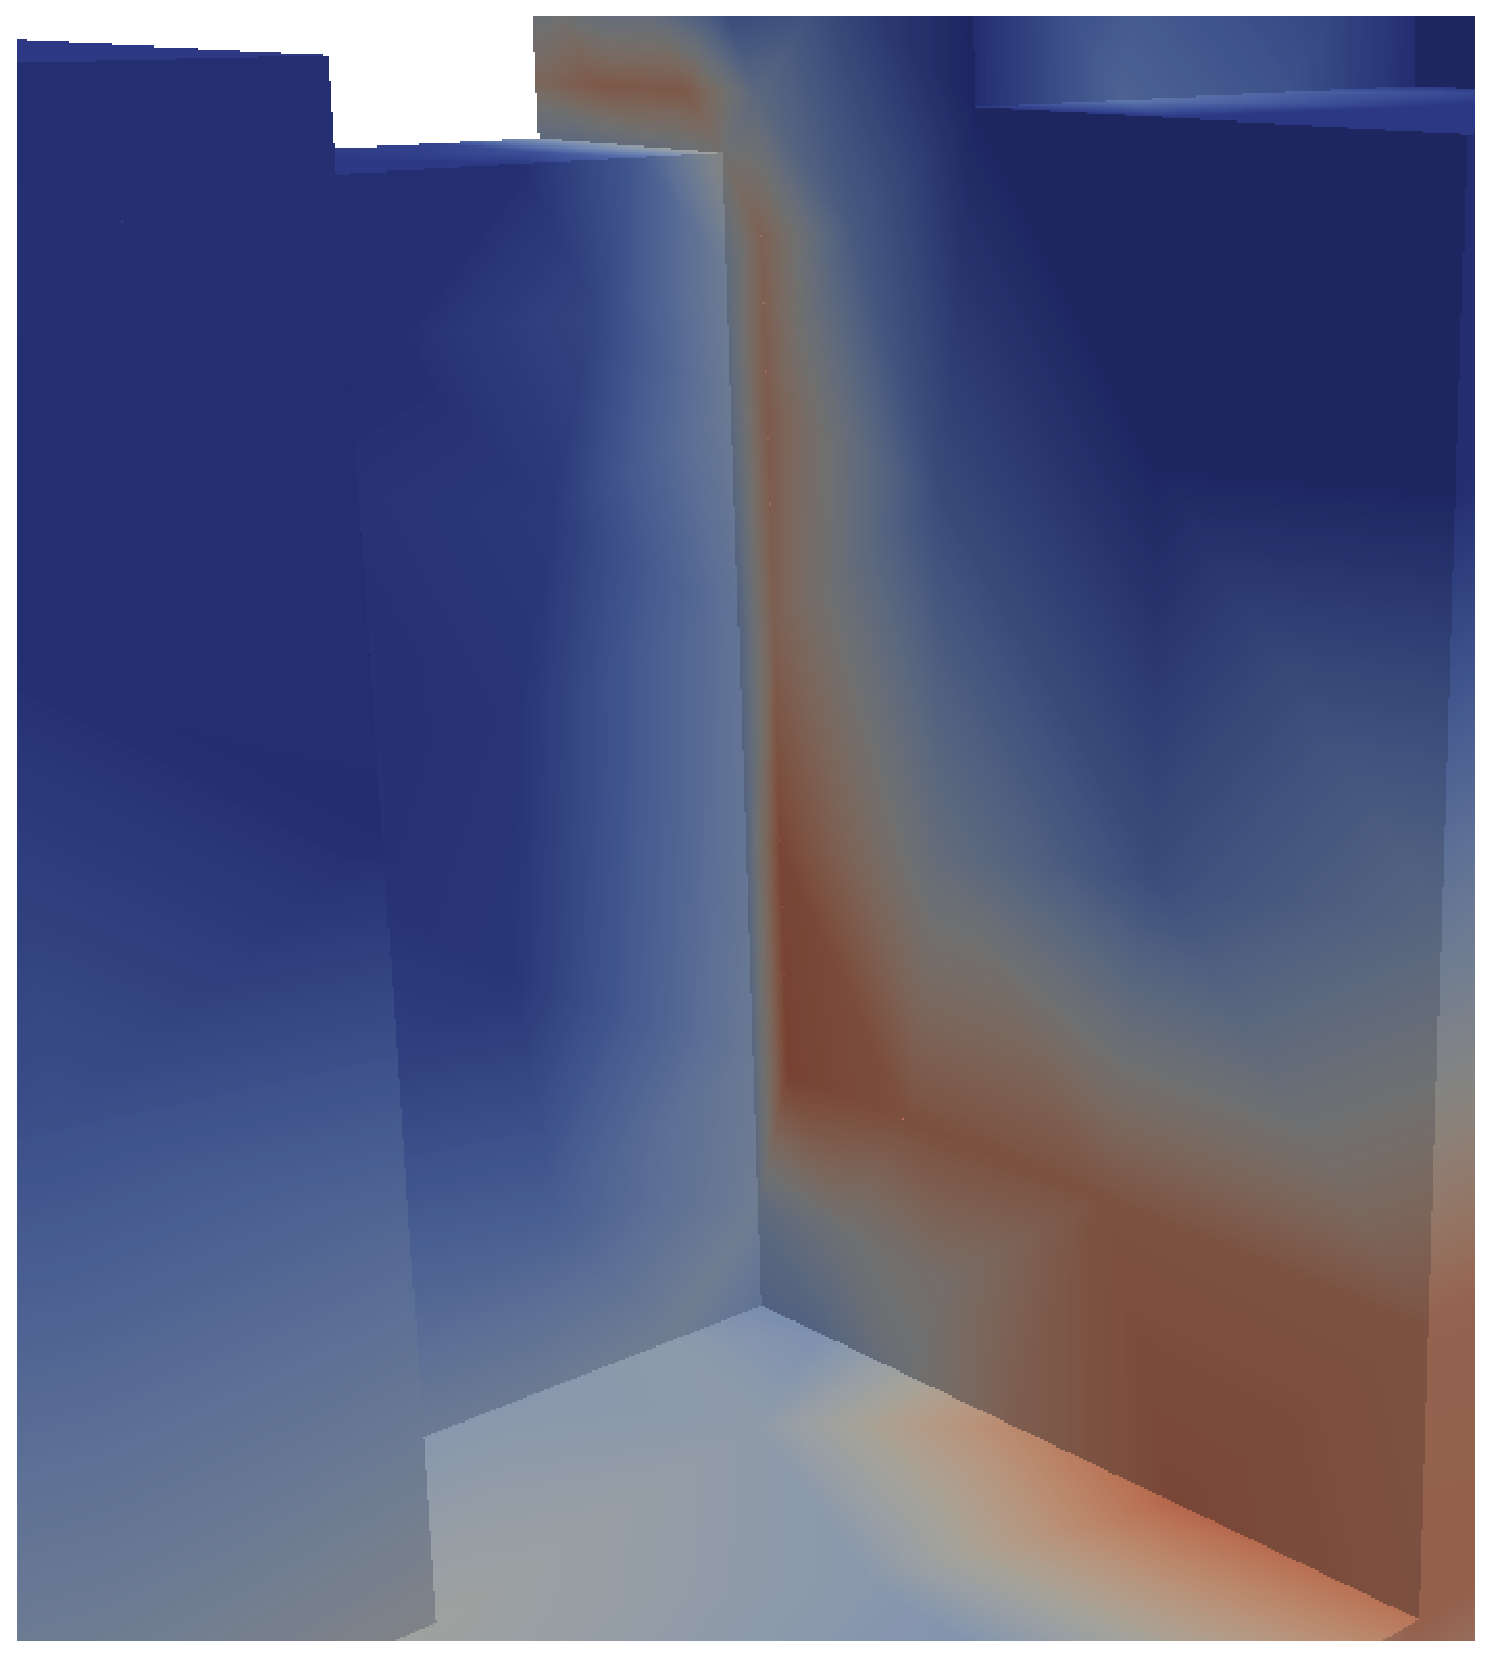
\includegraphics[scale=0.2]{figs/iter0_grad.eps}
                \caption*{Error indicator}
        \end{subfigure}
\end{figure}
   
\end{frame}


\begin{frame}[fragile]%[<+->]
  \frametitle{Refinement - Second Iteration}
  
\begin{figure}
        \centering
        \begin{subfigure}[b]{45mm}
                \centering
                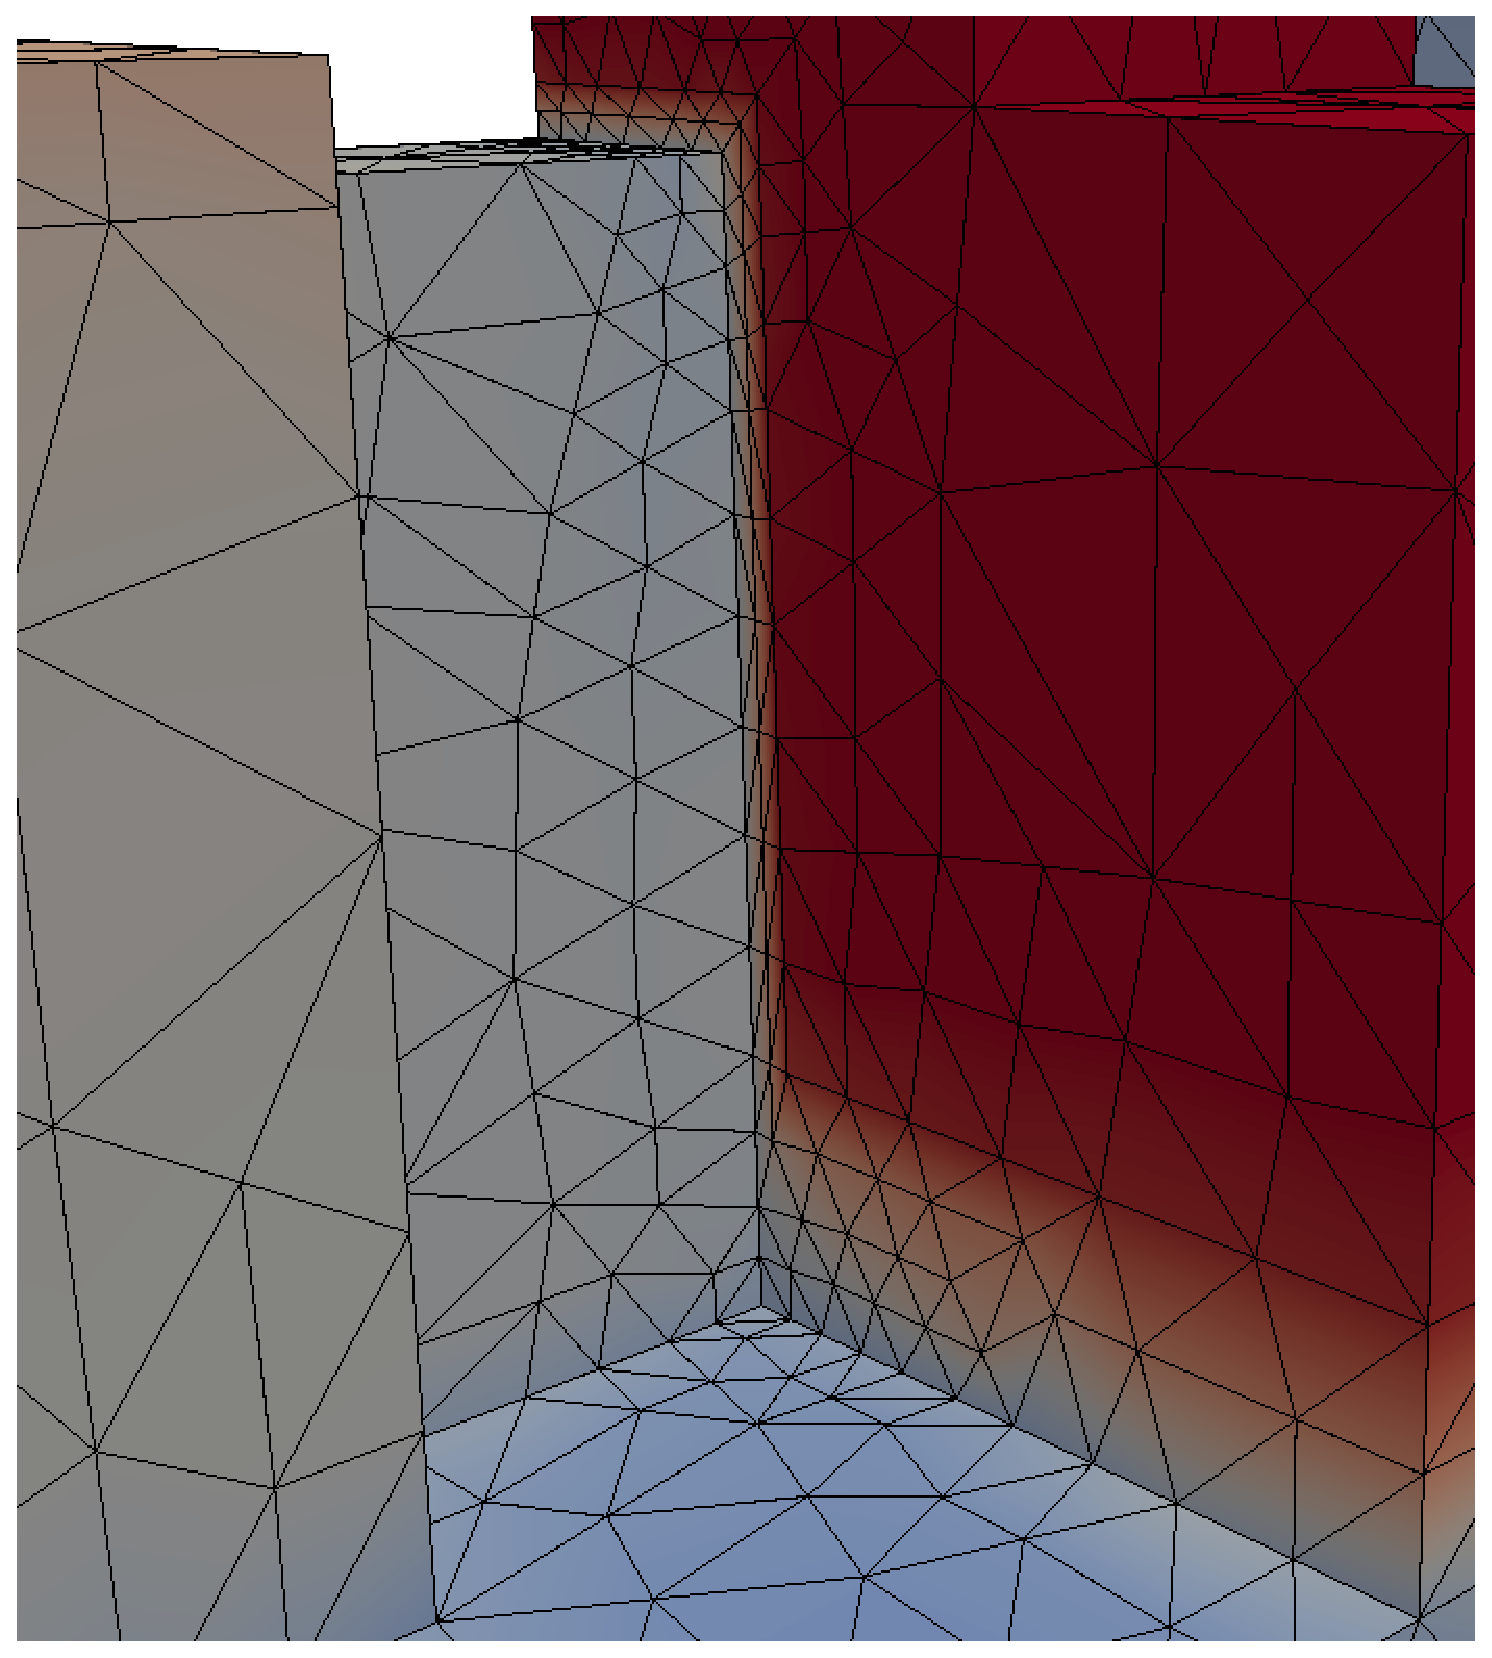
\includegraphics[scale=0.2]{figs/iter1_local.eps}
                \caption*{Potential}
        \end{subfigure}%
        \hspace{10mm}
        \begin{subfigure}[b]{45mm}
                \centering
                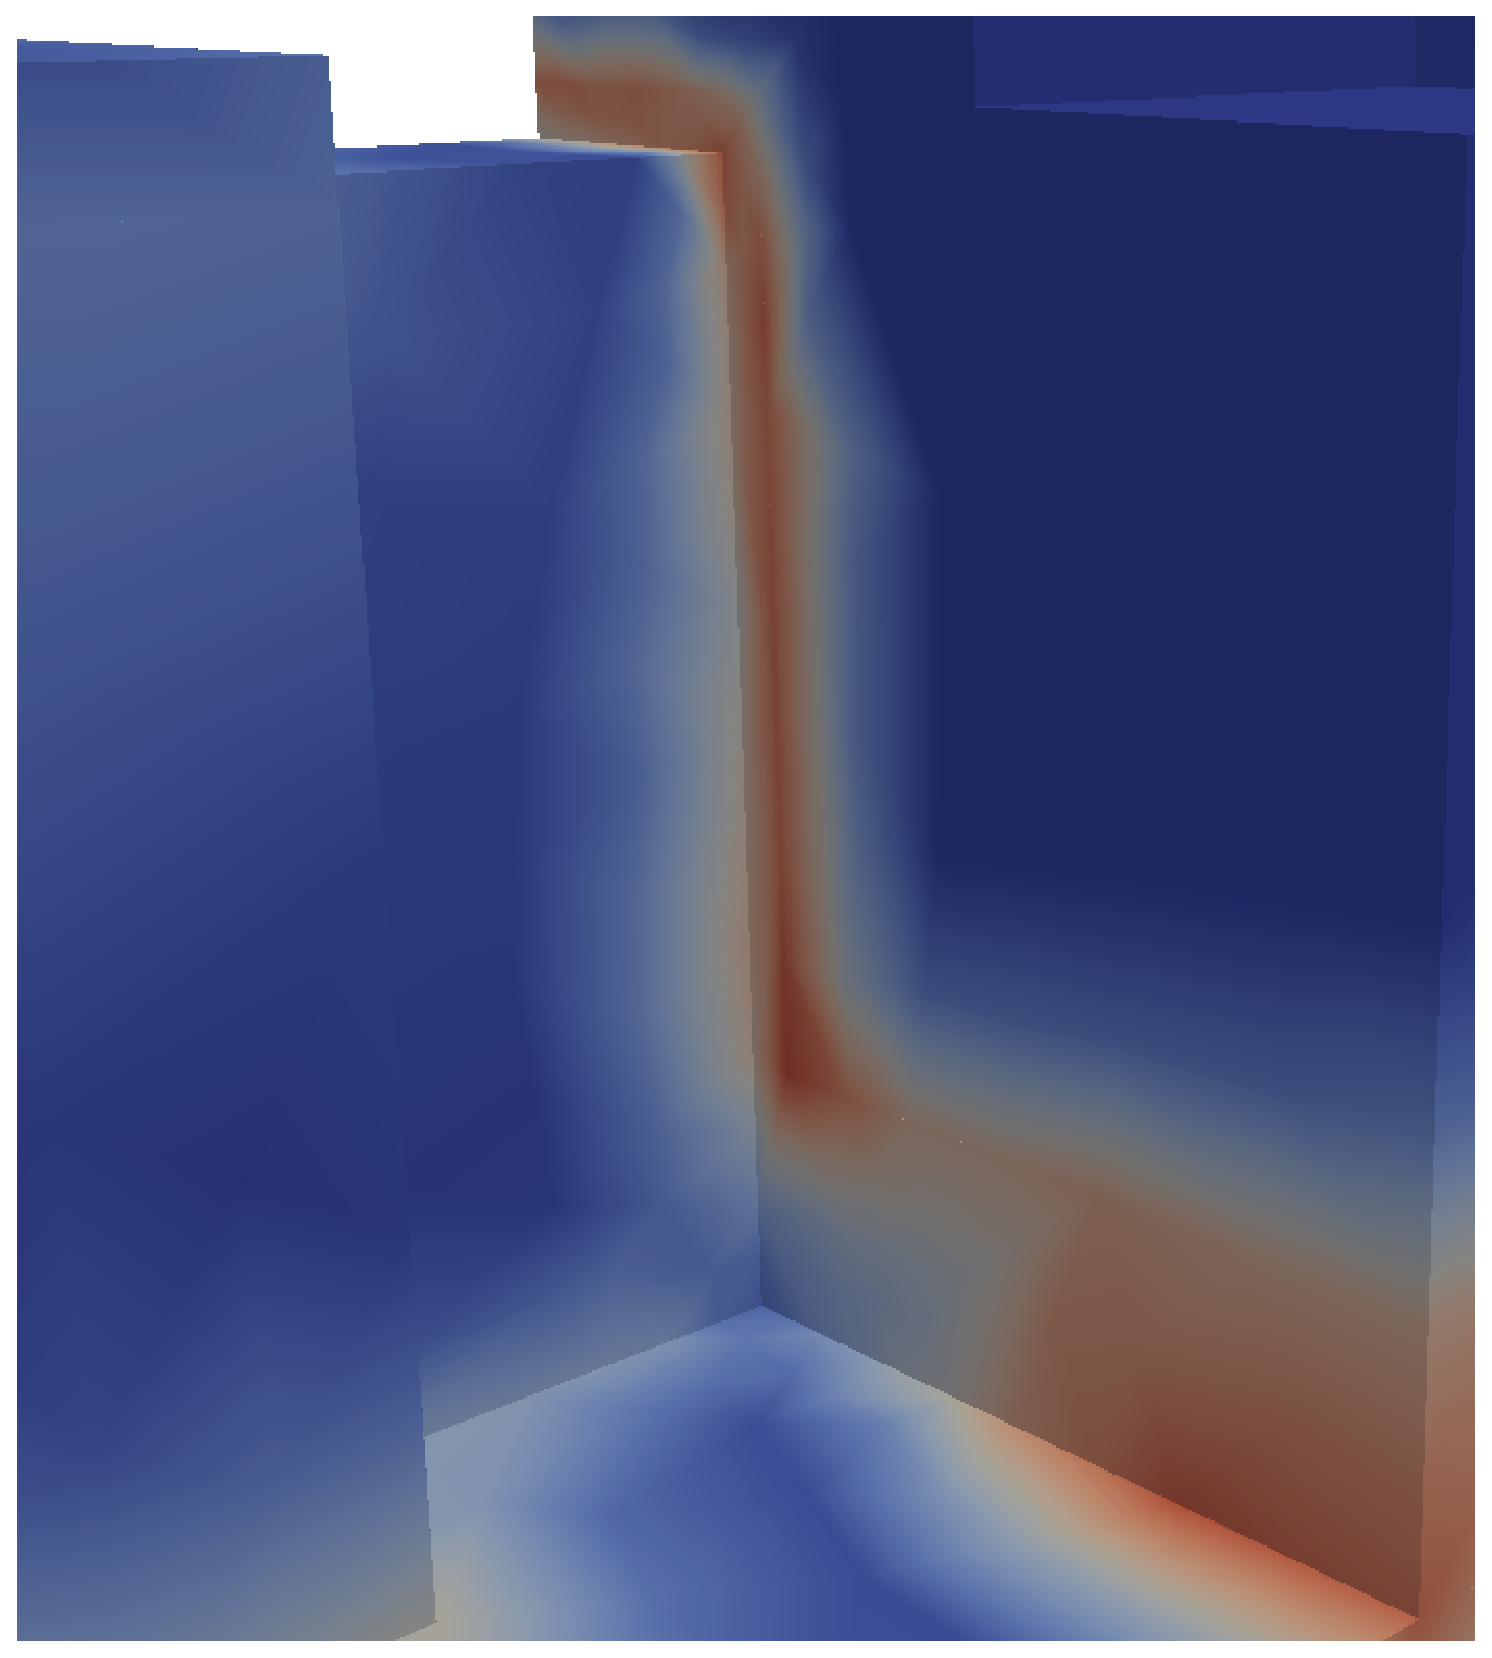
\includegraphics[scale=0.2]{figs/iter1_grad.eps}
                \caption*{Error indicator}
        \end{subfigure}
\end{figure}
   
\end{frame}



\begin{frame}[fragile]%[<+->]
  \frametitle{Refinement - Third Iteration}
  
\begin{figure}
        \centering
        \begin{subfigure}[b]{45mm}
                \centering
                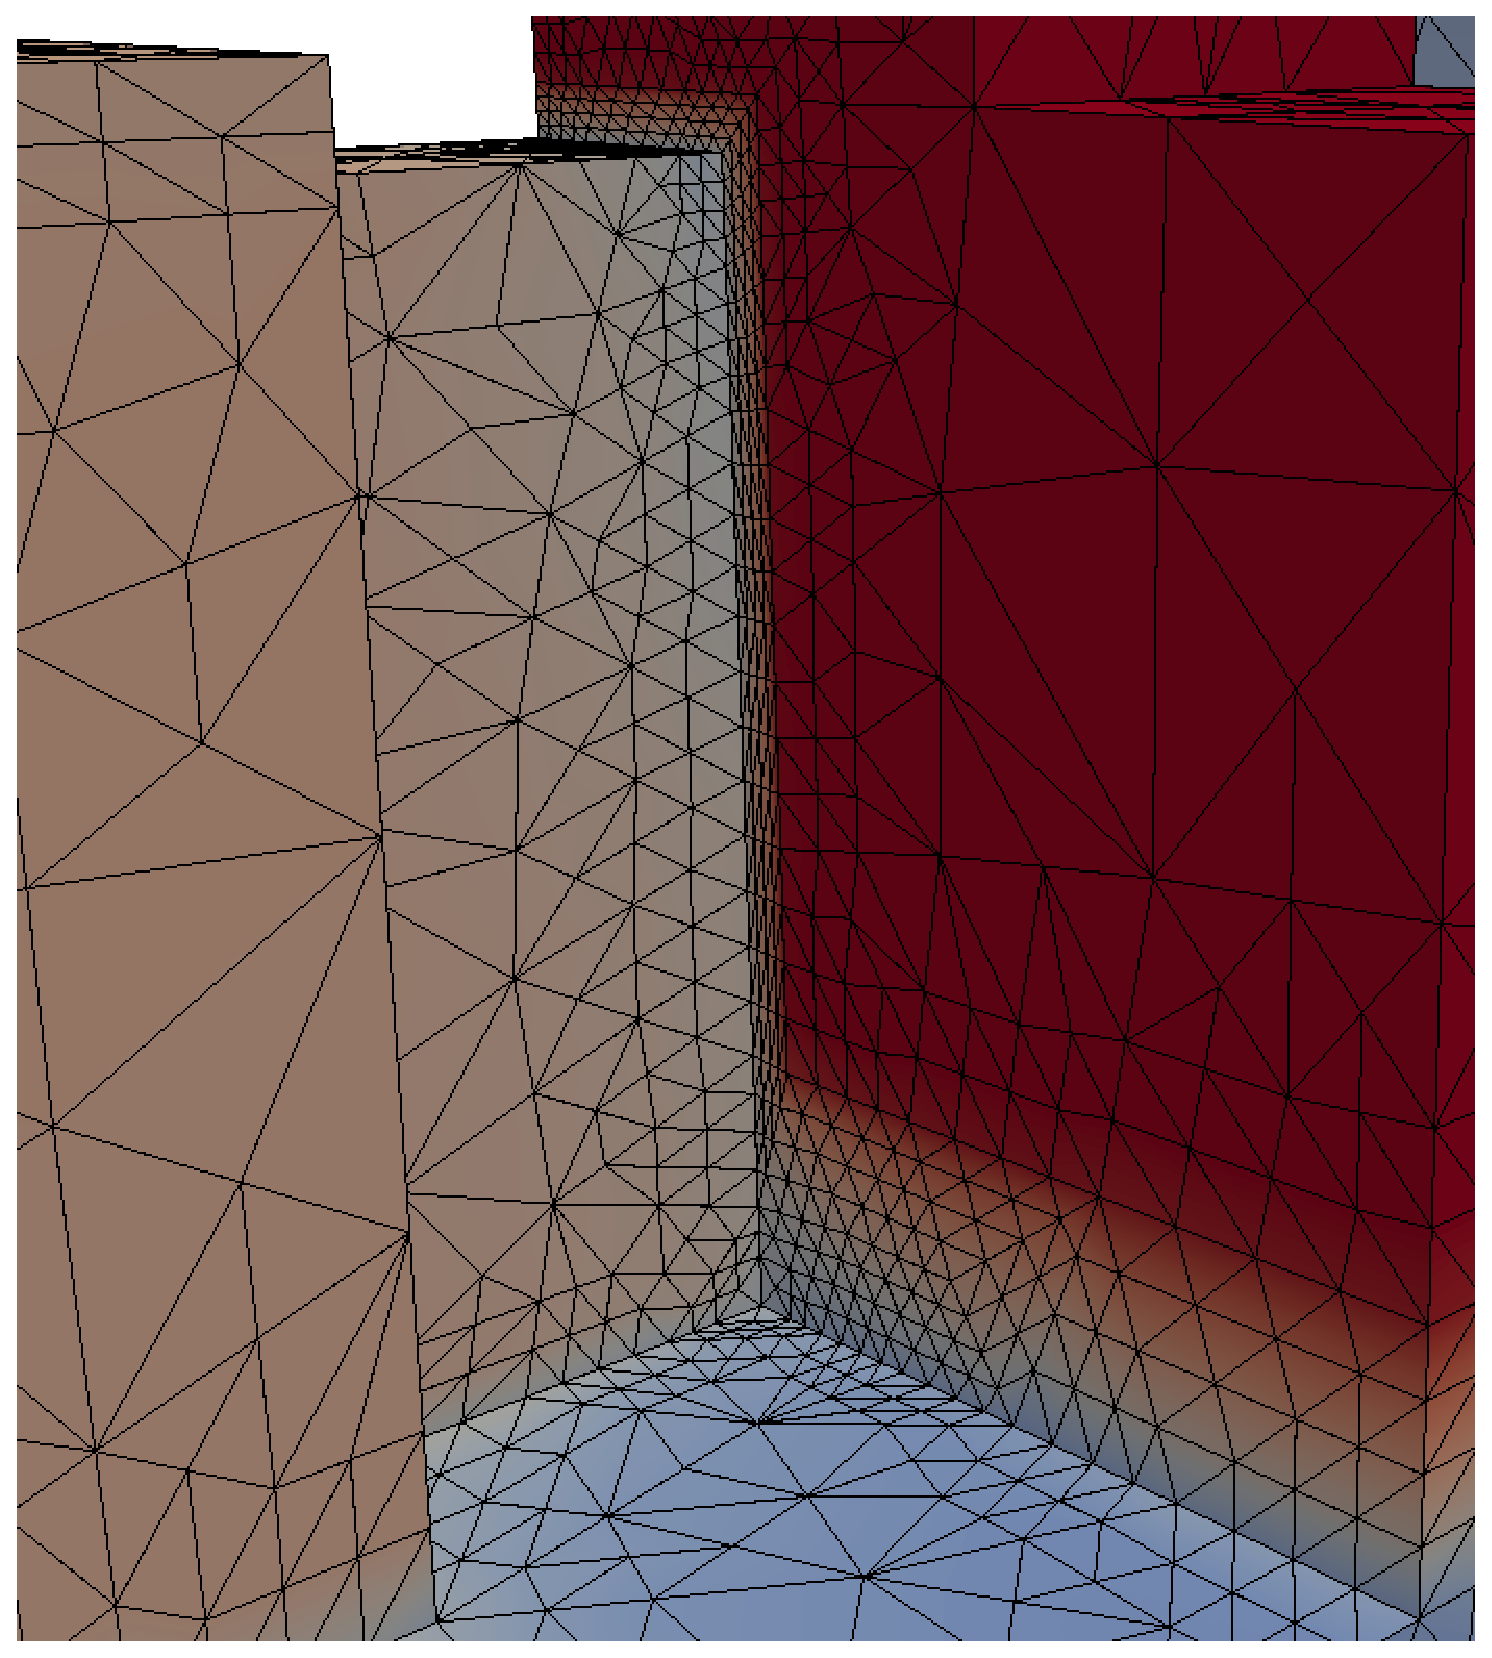
\includegraphics[scale=0.2]{figs/iter2_local.eps}
                \caption*{Potential}
        \end{subfigure}%
        \hspace{10mm}
        \begin{subfigure}[b]{45mm}
                \centering
                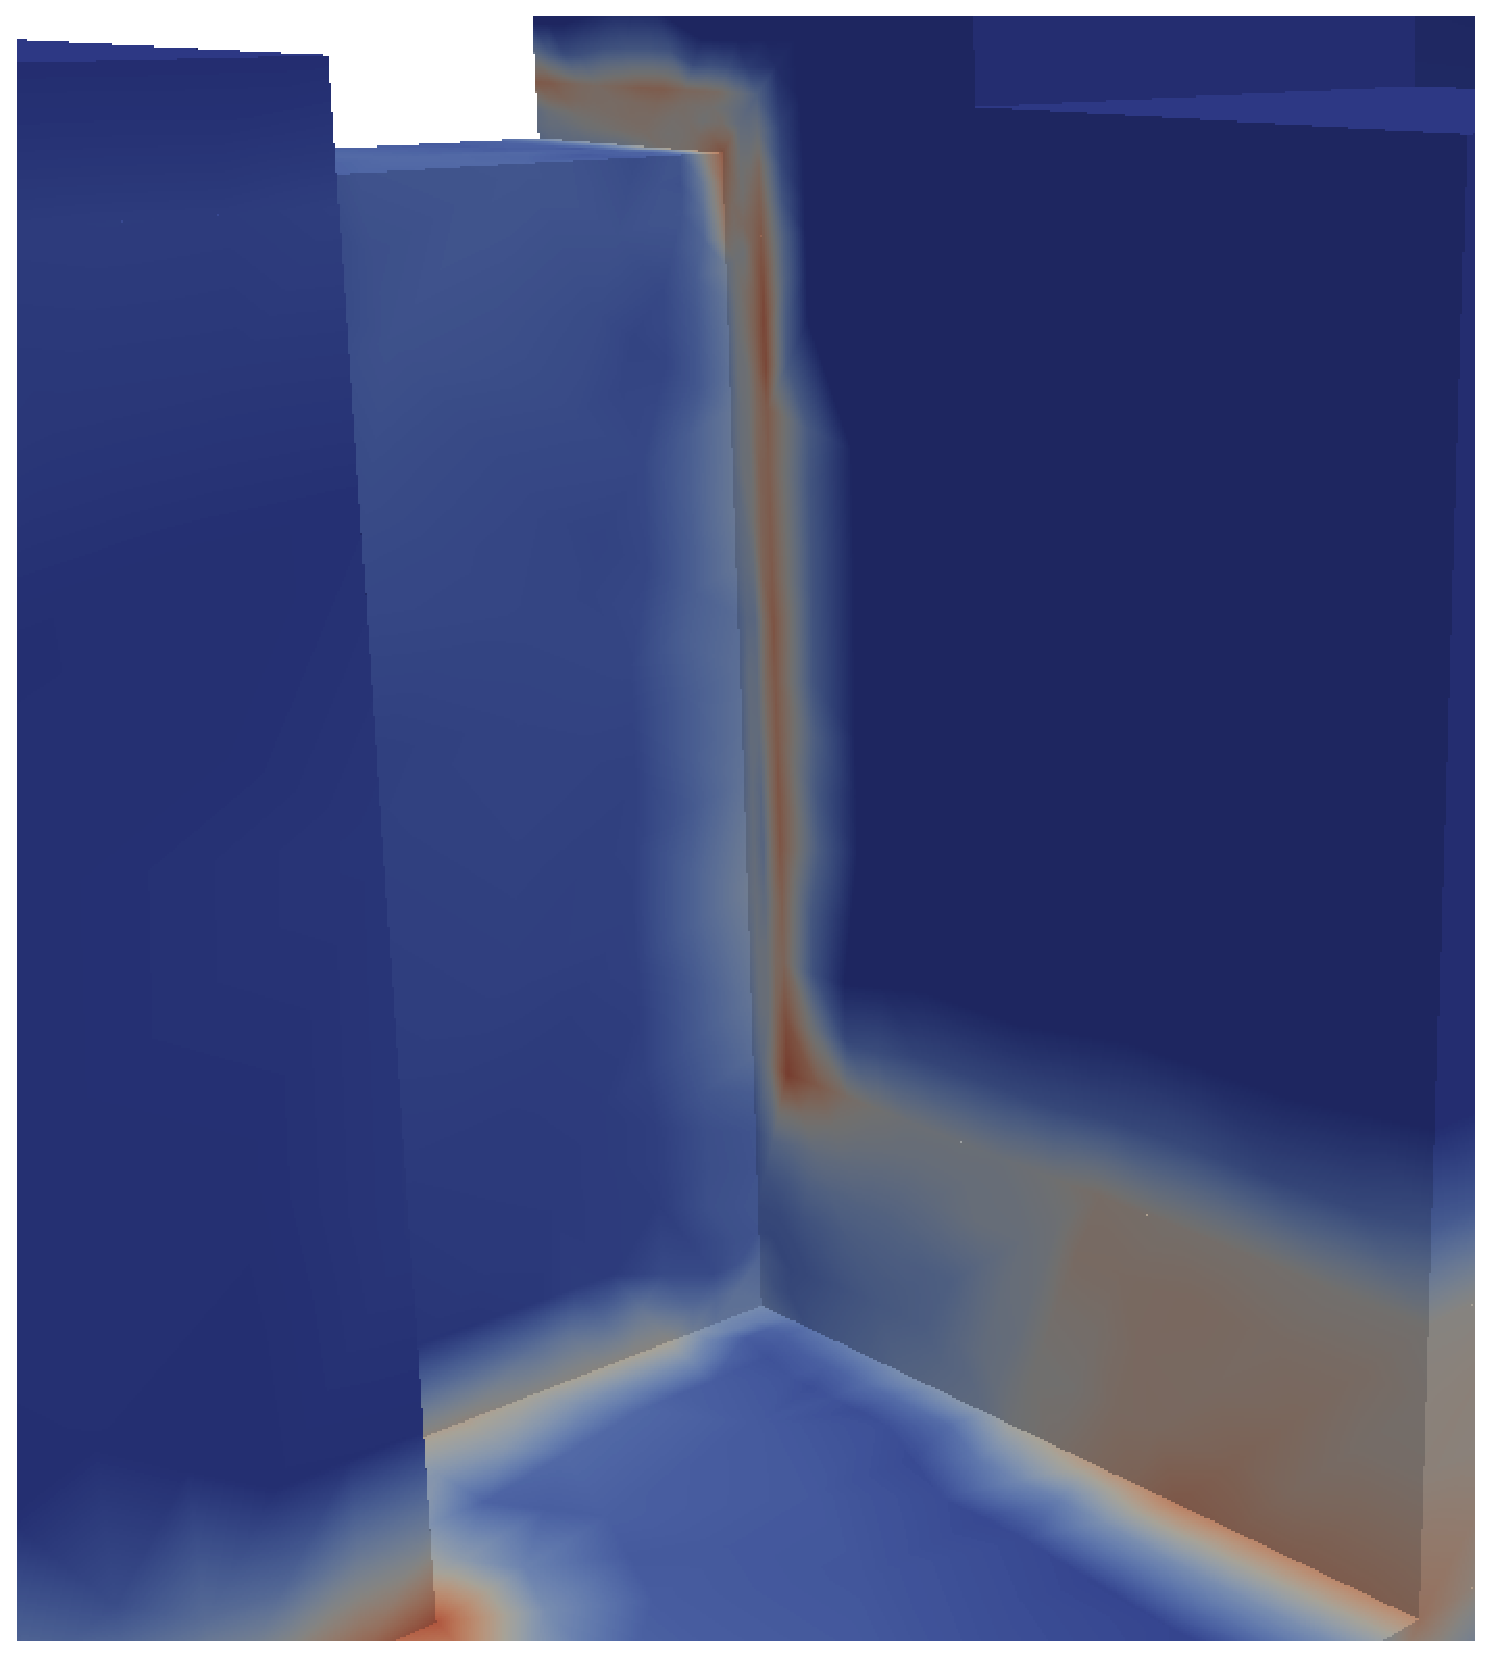
\includegraphics[scale=0.2]{figs/iter2_grad.eps}
                \caption*{Error indicator}
        \end{subfigure}
\end{figure}
   
\end{frame}



\begin{frame}[fragile]%[<+->]
  \frametitle{Drift Diffusion on 3D MOSFET Transistor}
  
\begin{figure}
        \centering
        \begin{subfigure}[b]{45mm}
                \centering
                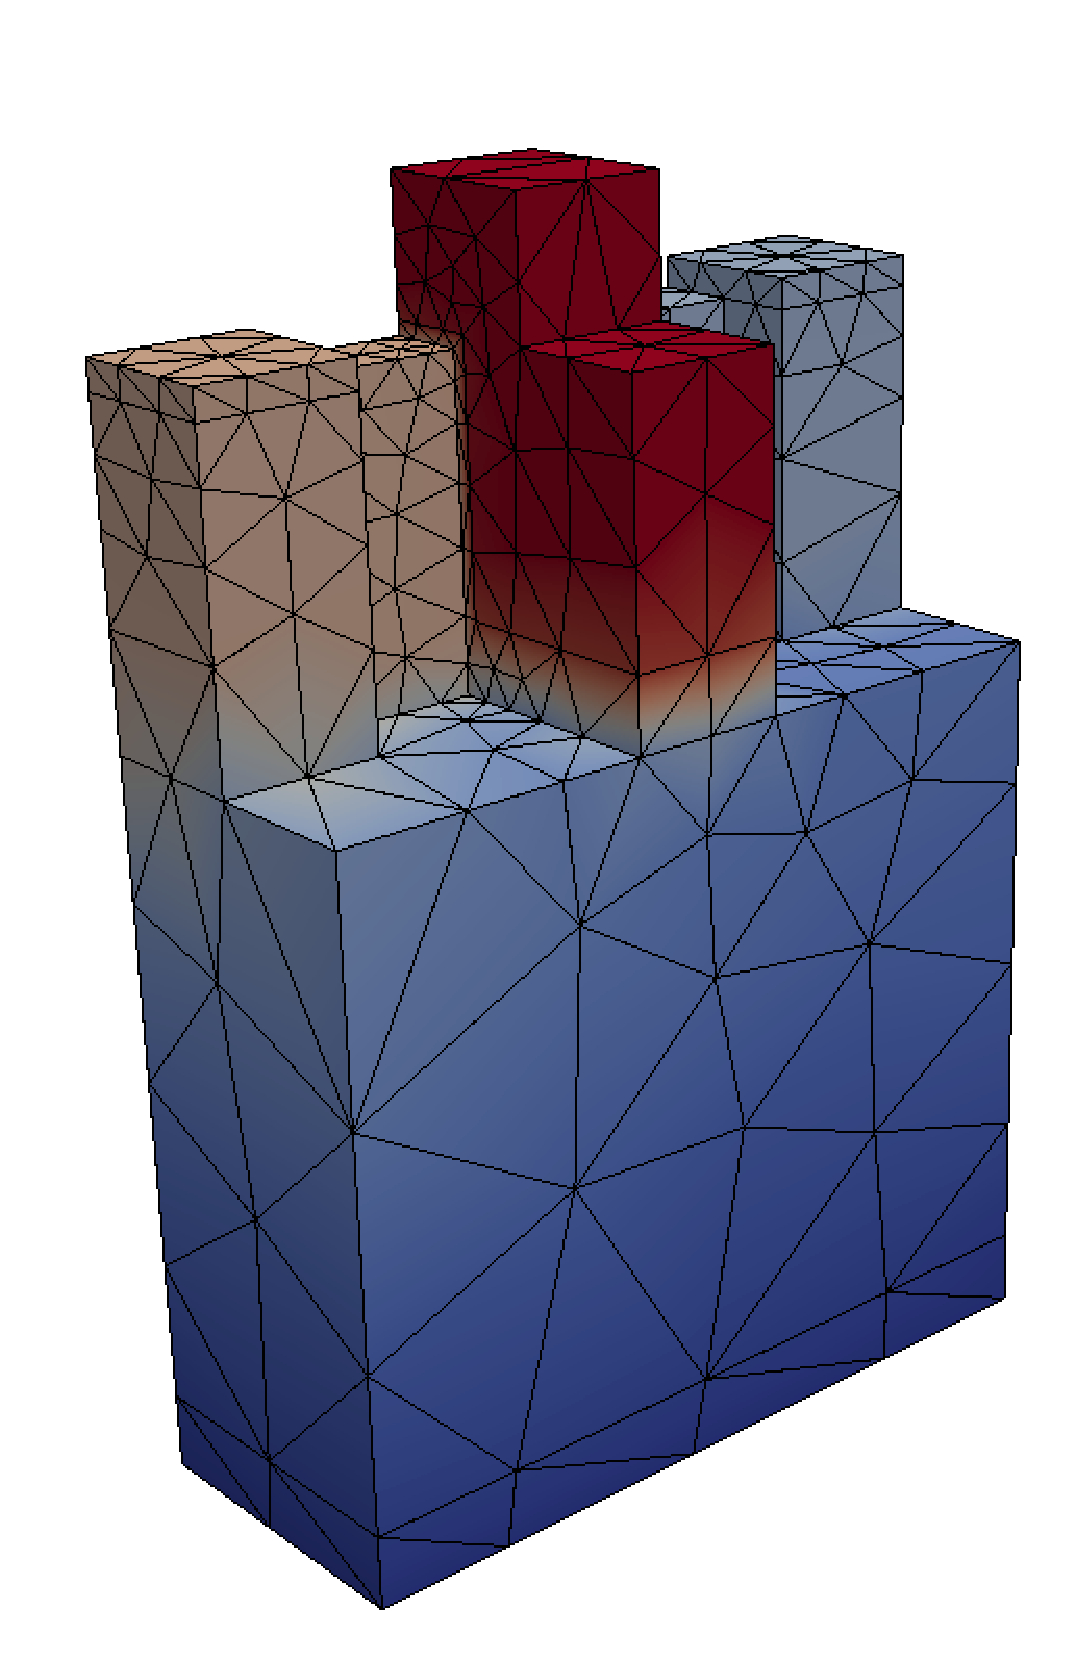
\includegraphics[scale=0.2]{figs/iter0_total.eps}
                \caption*{Initial mesh with 3200 cells}
        \end{subfigure}%
        \hspace{10mm}
        \begin{subfigure}[b]{45mm}
                \centering
                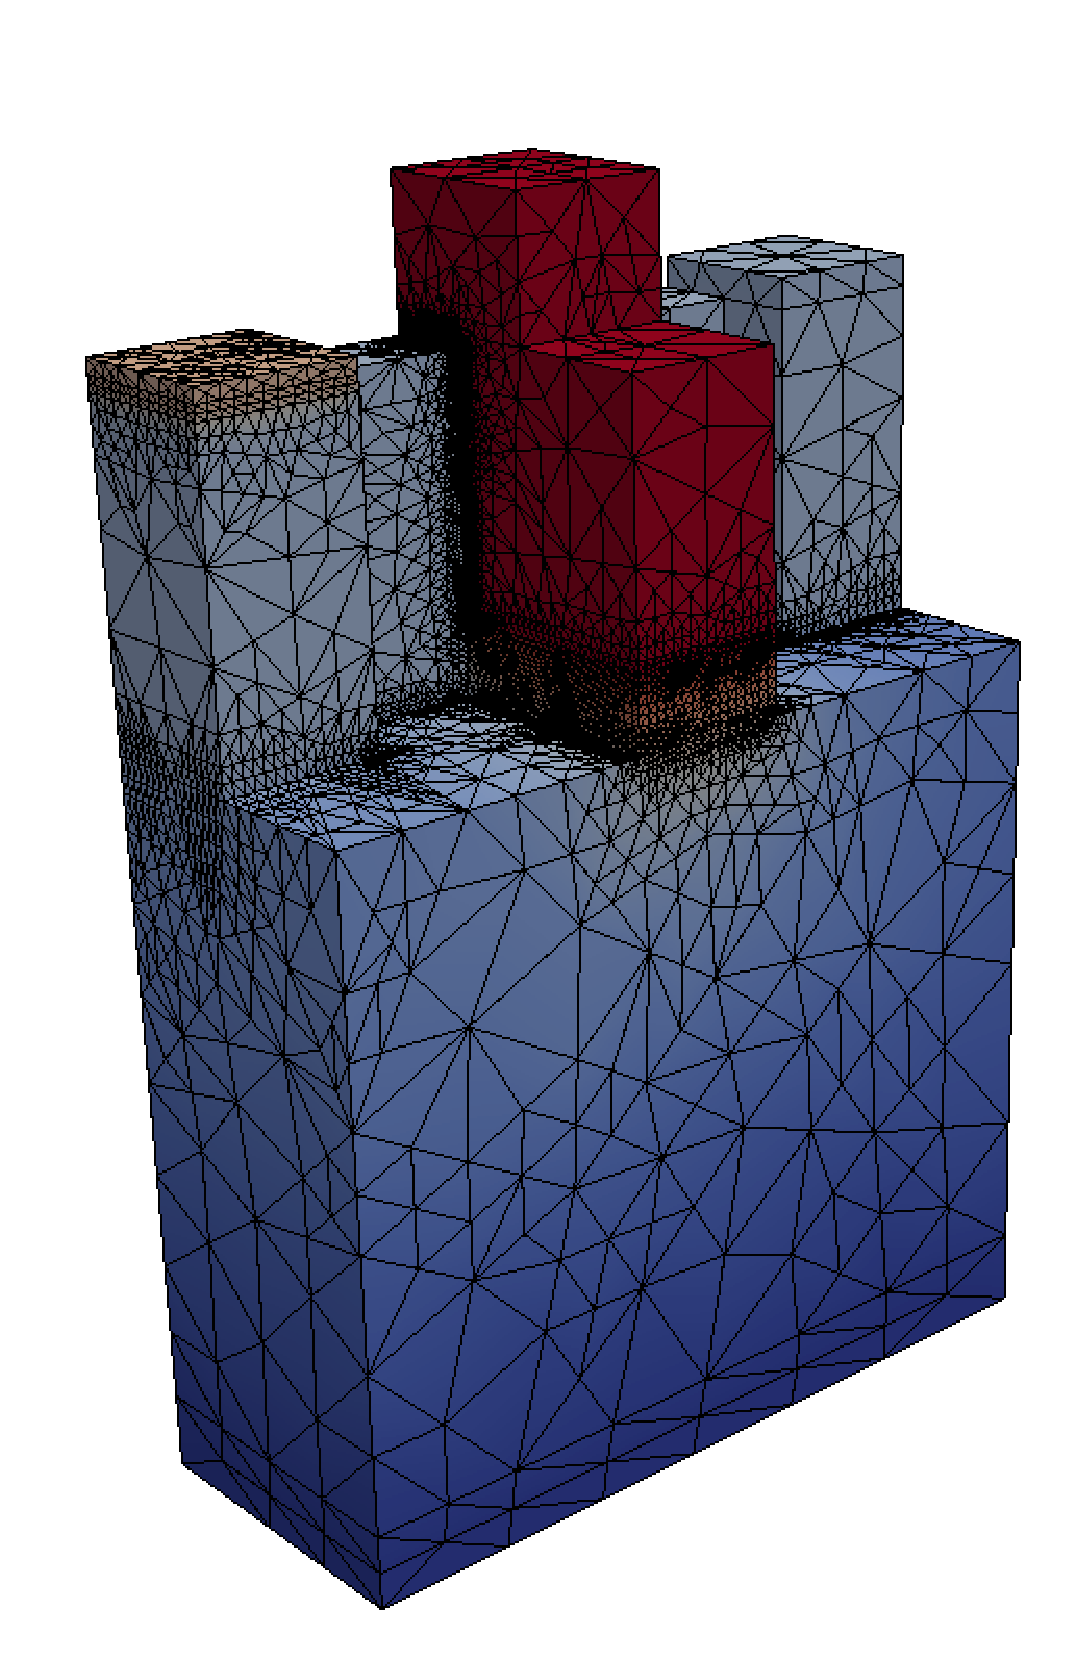
\includegraphics[scale=0.2]{figs/iter4_total.eps}
                \caption*{Iteration 4 with 467813 cells}
        \end{subfigure}
\end{figure}
   
\end{frame}




\begin{frame}[fragile]%[<+->]
  \frametitle{Use Case - Drift Diffusion on 3D MOSFET Transistor}
  
  \begin{block}{Cell count}
    \begin{table}
      \begin{tabular}{ r | r | r | r }
         iteration &  total cells  & bad cells & relative bad cells \\
         \hline
         1  &      3 200    &   2 082    &    65.06\% \\
         2  &      20 731   &   8 270    &    39.89\% \\
         3  &      103 366 &    40 302   &    38.99\% \\
         4  &       467 813  &  63 956   &    13.67\% \\
         5  &       1 349 050  & 15 144   &     1.12\% \\
         6  &      1 727 444   &  6 194    &    0.36\%
      \end{tabular}
    \end{table}
  \end{block}
  
\end{frame}


\begin{frame}[fragile]%[<+->]
  \frametitle{Use Case - Drift Diffusion on 3D MOSFET Transistor}
  
  \begin{block}{Cell count}
    \begin{table}
      \begin{tabular}{ r | r | r | r }
         iteration &  total cells  & bad cells & relative bad cells \\
         \hline
         \textbf{1}  &      \textbf{3 200}    &   \textbf{2 082}    &    \textbf{65.06\% }\\
         2  &      20 731   &   8 270    &    39.89\% \\
         3  &      103 366 &    40 302   &    38.99\% \\
         4  &       467 813  &  63 956   &    13.67\% \\
         5  &       1 349 050  & 15 144   &     1.12\% \\
         \textbf{6}  &      \textbf{1 727 444}   &  \textbf{6 194}    &    \textbf{0.36\%}
      \end{tabular}
    \end{table}
  \end{block}
  
\end{frame}





% ==============================================================================
\section{Conclusion}
\subsection{}

\begin{frame}[fragile]%[<+->]
  \frametitle{Conclusion}
  
  \begin{block}{Flexibility}
  \begin{itemize} \footnotesize
    \item Common interface \hspace{7.5mm} $\rightarrow$ \hspace{5mm} Easily change meshing kernel
    \item Abstract concepts \hspace{8mm} $\rightarrow$ \hspace{5mm} Write your code only once
    \item High configurability \hspace{5.8mm} $\rightarrow$ \hspace{5mm} Use arbitrary topological structures
    \item High extensibility \hspace{9mm} $\rightarrow$ \hspace{5mm} Write your own meshing algorithm
  \end{itemize}
  \end{block}

  \begin{block}{Status}
  \begin{itemize} \footnotesize
    \item Development release available at sourceforge
    \item http://viennamesh.sourceforge.net
  \end{itemize}
  \end{block}
\end{frame}

% ==============================================================================




\end{document}





